\documentclass{article}

\usepackage{geometry}
\geometry{
	a4paper,
	total={170mm,257mm},
	left=20mm,
	top=20mm,
}
\usepackage[utf8]{inputenc} % allow utf-8 input
\usepackage[T1]{fontenc}    % use 8-bit T1 fonts
\usepackage[hidelinks]{hyperref}       % hyperlinks
\usepackage{url}            % simple URL typesetting
\usepackage{tikz}
\usepackage{dsfont}
\usepackage{amsmath}
\usepackage{array}
\usepackage{authblk}
\usepackage{float}
\usepackage{rotating}
\usepackage[symbol]{footmisc}
\renewcommand{\thefootnote}{\fnsymbol{footnote}}
\usepackage{makecell}
\usepackage{ragged2e}
\usepackage{array}
\usepackage{longtable}

\usepackage{multirow, makecell}
\renewcommand{\arraystretch}{1.7}
\setlength{\tabcolsep}{12pt}

\graphicspath{{../../figures/}}

\renewcommand{\thefigure}{S\arabic{figure}}
\renewcommand{\thetable}{S\arabic{table}}

\title{Supplementary appendix to: \\ {\Large From SARS-CoV-2 Testing To COVID-19 Mortality: 
		Analysis of Swiss national surveillance data}}


\author[a,b,$\dagger$]{Julien Riou}
\author[a,$\dagger$]{Radoslaw Panczak}
\author[a]{Christian Althaus}
\author[b]{Christoph Junker}
\author[b]{Damir Perisa}
\author[b]{Katrin Schneider}
\author[a,c,d,*]{Matthias Egger}
\affil[a]{{\small Institute of Social and Preventive Medicine, University of Bern, Bern, Switzerland}}
\affil[b]{{\small Federal Office of Public Health, Liebefeld, Switzerland}}
\affil[c]{{\small Population Health Sciences, Bristol Medical School, University of Bristol, UK}}
\affil[d]{{\small Centre for Infectious Disease Epidemiology and Research, University of Cape Town, Cape Town, South Africa}}
\affil[$\dagger$] {{\small contributed equally}}
\affil[*] {{\small Corresponding  author (\texttt{matthias.egger@ispm.unibe.ch})}}


\begin{document}
	
	\maketitle
	
	\vspace{-3em}
	
	\tableofcontents
	
	\clearpage
	\section{Geocoding procedure}
	
	Geocoding of addresses was done under a contract between the FOPH and the Department of Environmental Sciences at ETH Zürich. Only address data were provided, no other information left the FOPH. Where no address but a ZIP code was available, we used the geocode corresponding to the ZIP code area. We linked each notification to the corresponding value of the Swiss neighbourhood index of SEP, using latitude and longitude of the home address. SEP values were grouped into deciles. Data were aggregated by canton (26 groups), sex (2 groups), age (9 groups, from 0-9 to 80 and older), SEP decile (10 groups) and epidemic wave (2 groups, before or after 8 June 2020) at the FOPH. The analysis dataset consisted of aggregated data only, and no individual data left the FOPH. 
	
\begin{table}[ht]
	\centering
	\caption{Results from the geocoding procedure.}
	\label{tab:geocode}
	\medskip
	\begin{tabular}{p{4.9cm}p{1.4cm}p{1.4cm}p{1.4cm}p{1.4cm}p{1.4cm}}
		\hline
		 &  Total tests & Positive tests & Hospitali-sations & ICU admissions & Deaths  \\ 
		\hline
	\textbf{Eligible} & 2,895,139 (100\%) & 488,531 (100\%) & 20,070 (100\%) & 1,983 (100\%) & 7,628 (100\%) \\ 
	\textbf{Geocoded and included} & 2,548,638 (88.0\%) & 423,656 (86.7\%) & 17,762 (88.5\%) & 1,785 (90.0\%) & 6,060 (79.4\%) \\ 
	\textbf{Geocoded based on}* &&&&& \\
	\hspace{1em}home address & 2,426,418 (95.2\%) & 410,561 (96.9\%) & 17,142 (96.5\%) & 1,655 (92.7\%) & 5,540 (91.4\%) \\ 
	\hspace{1em}ZIP code & 122,220 (4.8\%) & 13,095 (3.1\%) & 620 (3.5\%) & 130 (7.3\%) & 520 (8.6\%) \\ 
	
	\textbf{Geocodes corresponding to retirement or nursing homes}*& 53,784 (2.1\%) & 11,673 (2.8\%) & 674 (3.8\%) & 27 (1.5\%) & 1,864 (30.8\%) \\	
	\hline
	\multicolumn{6}{l}{\footnotesize{*Denominators for the calculation of percentages are all geocoded notifications.}}
	\end{tabular}
\end{table}


	\section{Extended methods}
	
	We analysed the association between SEP decile and counts of 1) SARS-CoV-2 tests, 2) positive cases, 3) COVID-19-related hospitalisations, 4) ICU admissions and 5) deaths with separate negative binomial regression models.  
	The procedure was similar for each of the five outcomes, except in the choice of denominator.
	Let $y_{i,j}$ be the count of the outcome of interest in a specific combination of SEP decile, age group, sex and period designed as $i$, and in canton $j$.
	There are $10 \times 9 \times 2 \times 2 = 360$ such combinations ($i \in \{1,\ldots,360\}$) in each of the $26$ cantons ($j\in \{1,\ldots,26\}$), so $y_{i,j}$ has a total length of $9360$. 
	In a first model (\underline{model 1}) we express $\eta_{i,j}$ the linear predictor corresponding to $y_{i,j}$ as
	\begin{equation}
		\eta_{i,j} = \exp\left[ \alpha + \beta\cdot\text{SEP}_{i,j}  + \log(\text{exposure}_{i,j}) \right],
		\label{eq:m1}
	\end{equation}
	where $\alpha$ is a global intercept, $\text{SEP}_{i,j}$ is the SEP decile (numerical value from 1 to 10), $\beta$ is a regression coefficient (i.e., $\exp(\beta)$ is the incidence rate ratio for one unit increase of SEP decile), and $\log(\text{exposure}_{i,j})$ is the offset.
	We refer to this model as unadjusted with SEP as a continuous variable.
	
	To assess whether including SEP as a continuous variable is adequate, we develop an alternative model (\underline{model 1'}) where 
	\begin{equation}
	\eta_{i,j} = \exp\left[ \alpha + \beta_2\cdot\text{SEP-2}_{i,j} + \beta_3\cdot\text{SEP-3}_{i,j} + \ldots + \beta_{10}\cdot\text{SEP-10}_{i,j}  + \log(\text{exposure}_{i,j}) \right],
	\label{eq:m2}
	\end{equation}
	where SEP-$k_{i,j}$ ($k \in \{2,\ldots,10\}$) is a dummy variable informing the count refers to individuals of SEP $k$.
	We compare this model to model 1 using model selection tools in order to assess whether the continuous assumption of model 1 is adequate.
	This continuous formulation is necessary to avoid inflating the number of parameters when introducing interactions (nine parameters are approximated with one).
	
	The next model (\underline{model 2}) introduces adjustment on age, sex, epidemic wave and an interaction between SEP and canton, with the linear predictor expressed as
	\begin{align}
		\eta_{i,j} = \exp[ \alpha_j + \beta_j\cdot\text{SEP}_{i,j}  + \gamma_1\cdot\text{Age}_{2,i,j}
		+ \ldots + \gamma_8\cdot\text{Age}_{9,i,j} + \delta\cdot\text{Sex}_{i,j} + \\ \nonumber \zeta\cdot\text{Wave}_{i,j} + \iota\cdot\text{SEP}_{i,j}\cdot\text{Period}_{i,j}  +
		\log(\text{exposure}_{i,j}) ].
		\label{eq:m3}
	\end{align}
	In this formulation, the intercept $\alpha_j$ can vary by canton (this type of formulation can be referred to as a ``random intercept'').
	The regression coefficient for SEP $\beta_j$ is also allowed to vary by canton (``random slope'').
	This implies that there are now 26 parameters $\alpha_j$ and 26 parameters $\beta_j$ in the model, themselves controlled by hyperparameters:
	\begin{align}
		\alpha_j & = \mu_{\alpha} + \sigma_{\alpha}\cdot a_j \text{ \hspace{2.05em}with } a_j \sim \mathcal{N}(0,1) \\ 
		\beta_j & = \mu_{\beta} + \sigma_{\beta}\cdot b_j \text{ \ \hspace{2em}with } b_j \sim \mathcal{N}(0,1) 
		\label{eq:m3b}
	\end{align}
	Note that because of the exponential link function, the estimated parameters $a_j$ and $b_j$ have a multiplicative effect.
	The remaining elements of equation  are regression coefficients for the age groups (in 9 groups, from 0-9 to 80+), for the sex and for the epidemic wave (2 waves). 
	
	Following the same principles, we also develop a last model (\underline{model 3}) that includes interactions between SEP and age group, SEP and sex and SEP and epidemic wave.
	
	In all models, the likelihood can be expressed as
	\begin{equation}
		\Pr(\theta | y) = \prod_i \prod_j  \text{negative-binomial}(y_{i,j} | \eta_{i,j},\phi),
	\end{equation}
	where $\phi$ is the overdispersion parameter and $\theta$ corresponds to the set of all parameters and hyperparameters to be estimated.
	The models are implemented in \texttt{R} using package \texttt{rstanarm} \cite{goodrich2020brilleman}.
	We select weakly-informative priors for all parameters, that is normal distributions with mean 0 and standard deviation 2.5 for intercept and slope parameters and exponential distributions with rate 1 for overdispersion parameters.
	All code is available at \url{https://github.com/RPanczak/ISPM_COVID-SEP/}.
	
	
	\section{Extended results}
	
	\subsection{Model selection}
	
	Model selection was based on the left-one-out information criterion (LOOIC) \cite{vehtari2017practical}. 
	This quantity evaluates the pointwise out-of-sample prediction accuracy from a fitted Bayesian model using the log-likelihood evaluated at the posterior simulations of the parameter values.
	LOOIC values can be compared across models fitted to the same dataset by computing the pointwise difference in predictive accuracy. 
	As for other information criterions such as the Akaike Information Criterion, a decrease in LOOIC corresponds to a better model fit.
	Rather than using a fixed threshold, LOOIC differences must be assessed with regards to their uncertainty, for instance using the standard error.
	A common approach is to consider a model as better than another if the LOOIC difference is negative and greater than two times its standard error.
	
	Table \ref{tab:s2} present LOOIC estimates for models 1 to 3 and LOOIC differences with model 1 as a reference. 
	We see that the difference between models 1 and 2 is quite small overall, and generally positive, meaning that model 1 generally has a better fit than model 1'. 
	On the other hand, model 2 is clearly an improvement over model 1.
	
	
	\begin{table}[H]
		\centering
		\caption{Model selection based on left-one-out information criterion (LOOIC). Three models are compared: unadjusted model with SEP as a continuous variable (model 1), unadjusted model with SEP as a discrete variable (model 1') and adjusted model with SEP as a continuous variable (model 2, adjustment on age, sex, epidemic period and canton).}
		\label{tab:s2}
		\medskip
		\scalebox{.8}{\begin{tabular}{p{2.4cm}p{2.5cm}p{2.3cm}p{2.2cm}p{2.2cm}p{2.3cm}p{2.2cm}}
				\hline
				Outcome & Denominator & LOOIC (se) for model 1 & LOOIC (se) for model 1' & Difference (se) with model 1 & LOOIC (se) for model 2 & Difference (se) with model 1 \\ 
				\hline
				Total tests & Per population & 98,178 (459) & 98,186 (459) & +8 (3) & 73,475 (460) & -24,703 (224) \\ 
				Positive tests & Per population & 72,155 (383) & 72,165 (383) & +10 (3) & 54,414 (380) & -17,741 (193) \\ 
				Positive tests & Per test & 45,346 (374) & 45,336 (373) & -10 (11) & 34,059 (373) & -11,287 (176) \\ 
				Hospitalisations & Per population & 27,948 (311) & 27,964 (312) & +16 (4) & 18,701 (229) & -9,247 (172) \\ 
				Hospitalisations & Per test & 18,840 (286) & 18,853 (287) & +13 (4) & 12,234 (209) & -6,606 (136) \\ 
				Hospitalisations & Per positive test & 25,108 (248) & 25,119 (248) & +10 (4) & 17,699 (203) & -7,409 (135) \\ 
				ICU admissions & Per population & 8,455 (196) & 8,469 (197) & +14 (3) & 5,897 (144) & -2,559 (99) \\ 
				ICU admissions & Per test & 5,967 (165) & 5,979 (166) & +11 (4) & 4,031 (121) & -1,937 (83) \\ 
				ICU admissions & Per positive test & 7,950 (182) & 7,962 (182) & +12 (4) & 5,678 (137) & -2,272 (91) \\ 
				Deaths & Per population & 13,858 (292) & 13,871 (292) & +14 (3) & 8,028 (189) & -5,830 (147) \\ 
				Deaths & Per test & 9,419 (243) & 9,432 (244) & +13 (3) & 5,206 (158) & -4,213 (126) \\ 
				Deaths & Per positive test & 12,525 (249) & 12,539 (249) & +13 (2) & 6,889 (159) & -5,637 (138) \\ 
				\hline
		\end{tabular}}
	\end{table}
	
	\subsection{Model fit}
	\label{sec:fit}
	Figure \ref{fig:fig-fit} shows the posterior predictive check of the adjusted model (model 2) applied to all relevant combinations of outcome and denominator.
	The fit is generally very good, with most data point falling into the 95\% prediction intervals.
	
	
	\begin{figure}[H]
		\centering
		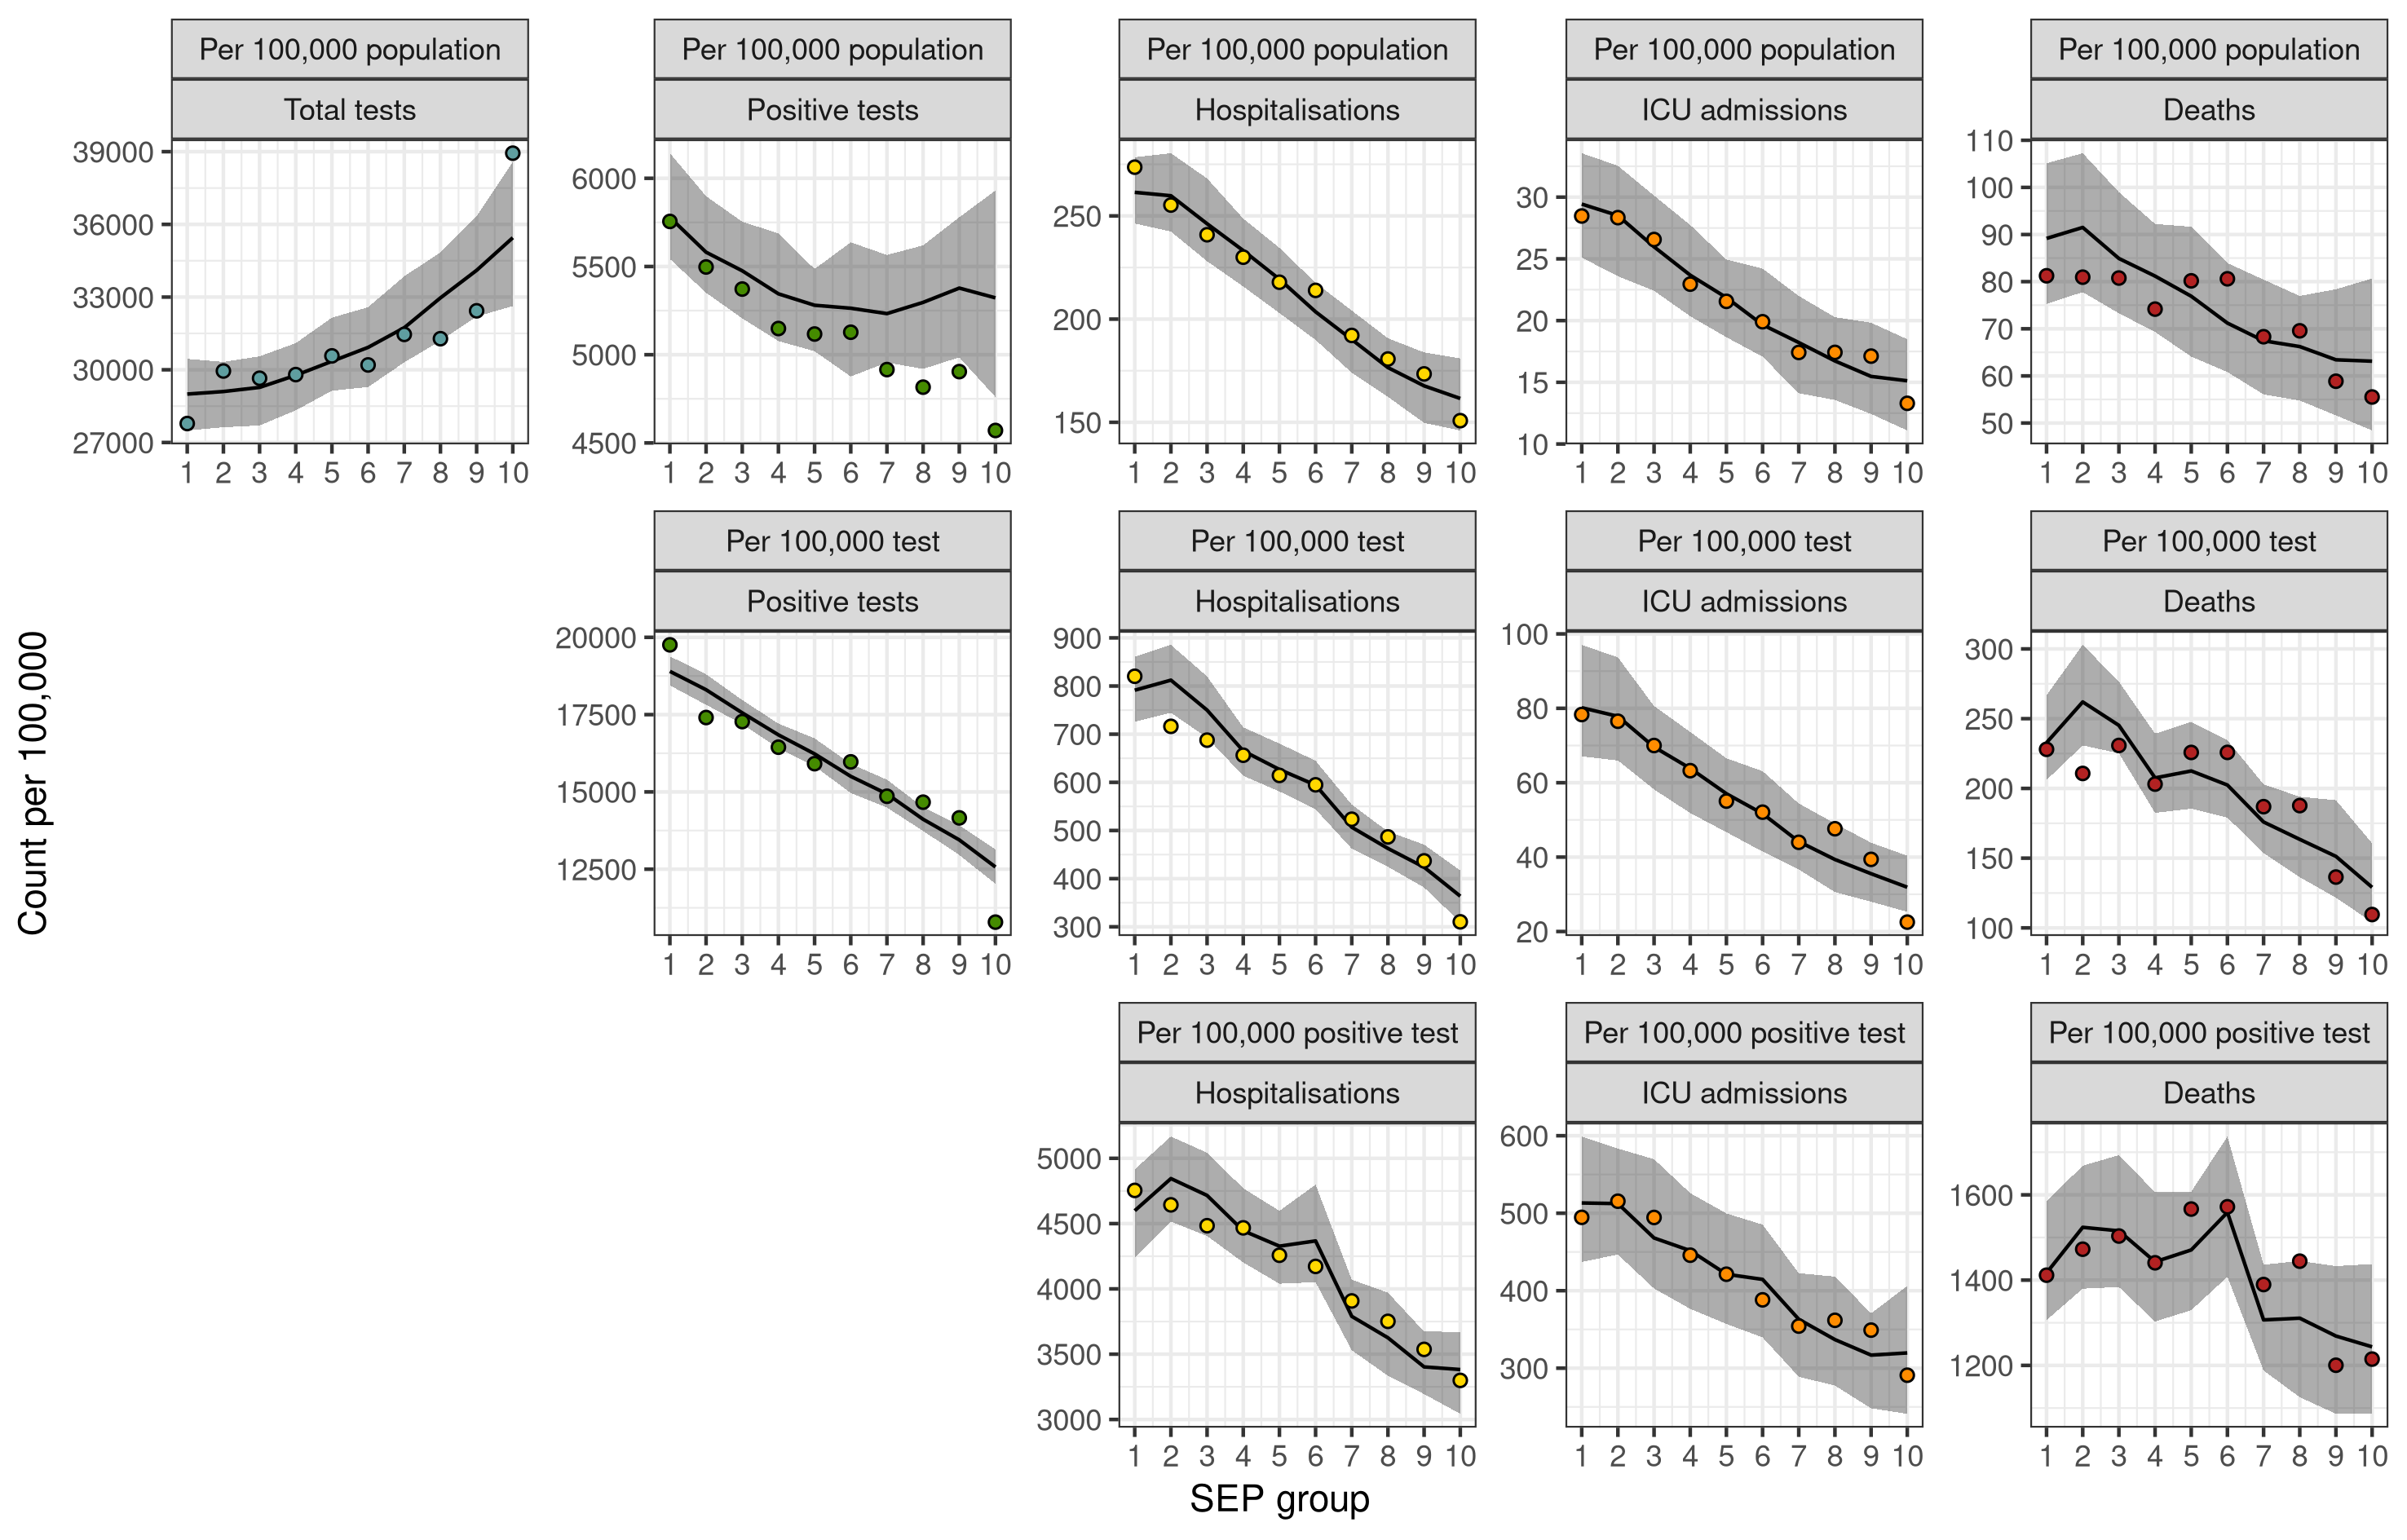
\includegraphics[width=\linewidth]{suppfigure_model_fit_adjusted.png}
		\caption{Fit of the models adjusted for age, sex, epidemic wave and canton. Circles show data points, the line and shaded area show the corresponding model prediction (median and 95\% prediction interval).}
		\label{fig:fig-fit}
	\end{figure}
	
	We spot potential issues in three areas.
	First, the number of total tests per 100,000 population is not well-predicted by the model in the highest SEP decile, suggesting that the continuous formulation could be inadequate.
	Still, LOOIC comparisons between model 1 (continuous) and model 1' (discrete) in Table \ref{tab:s2} don't suggest an advantage in using a discrete formulation. 
	Moreover, a discrete formulation would lead to huge inflation of the number of parameters when including interactions. 
	We decide to continue with the continuous formulation and consider testing in the 10th decile as an outlier.
	
	Second, the number of positive tests per 100,000 tests is also not well-predicted in the highest SEP decile. 
	This issue mirrors the previous one, but this time there is an indication that the discrete formulation might fit better (LOOIC difference -10 with a standard error of 11).
	Still, considering the difficulty posed by using 9 parameters instead of 1 for the effect of SEP, we go ahead with the continuous approach.
	
	Third, the number of positive tests per 100,000 population is not well-described for the SEP deciles 7, 8, 9 and 10.
	This issue is not related to the continuous formulation, as the comparison between models 1 and 2 shows.
	Rather, this discrepancy comes from an interaction between the effect of SEP and the epidemic wave, as detailed in section \ref{sec:period}.

	
	
	\subsection{Socio-economic position}
	
	Table \ref{tab:s3} presents additional results about models 1, 2 and 3. 
	We present incidence rate ratios (IRRs) per SEP decile for models 1, corresponding to $\exp(\beta)$ in equation \ref{eq:m1}.
	For model 2, the IRRs per SEP decile correspond to the average effect of one SEP decile across cantons, $\exp(\mu_{\beta})$ in equation \ref{eq:m3b}.
	In the models using a continuous formulation (1 and 3), IRRs for the 10th decile of SEP compared to 1st can be computed from the IRRs per SEP decile to the power of 9.
	For the model with a discrete formulation (model 1'), the IRRs for the 10th decile of SEP compared to 1st correspond to $\exp(\beta_{10})$ in equation \ref{eq:m2}.
	
	IRRs per SEP decile are all similar between models 1 and 3, suggesting that while the adjustment on age, sex, epidemic wave and canton clearly improved the model fit (Table \ref{tab:s2}), the association between SEP and each outcome remain consistent.
	Comparing the IRRs for the 10th decile of SEP compared to the 1st allows comparing all three models, and again assess the adequacy of the continuous formulation. 
	The estimates are mostly in agreement, comforting our approach.
	We observe a difference in the total tests per population and in positive tests per tests, corresponding to outliers in the 10th SEP decile as discussed above.
	
	
	
	\begin{table}[H]
		\centering
		\caption{Association of deciles of neighbourhood index of socioeconomic position (SEP) with five outcomes related to SARS-CoV-2 surveillance and care: total tests, positive tests, hospitalisations, intensive care unit (ICU) admissions and deaths. Three denominators are considered accordingly: population, total tests and positive tests. Three models are considered: unadjusted model with SEP as a continuous variable (model 1), unadjusted model with SEP as a discrete variable (model 1') and adjusted model with SEP as a continuous variable (model 2, adjustment on age, sex, epidemic period and canton).}
		\label{tab:s3}
		\medskip
		\scalebox{.75}{\begin{tabular}{p{2.4cm}p{2.5cm}p{2.5cm}p{2.5cm}p{2.5cm}p{2.5cm}p{2.5cm}}
			\hline
				Outcome & Denominator & IRR per SEP decile for model 1 & IRR for 10th decile compared to 1st for model 1 & IRR for 10th decile compared to 1st for model 1' & IRR per SEP decile for model 2 & IRR for 10th decile compared to 1st for model 2 \\ 
			\hline
			Total tests & Per population & 1.02 (1.01-1.03) & 1.20 (1.07-1.33) & 1.30 (1.12-1.52) & 1.02 (1.01-1.04) & 1.21 (1.05-1.40) \\ 
			Positive tests & Per population & 0.99 (0.98-1.00) & 0.92 (0.84-1.02) & 0.90 (0.78-1.04) & 1.00 (0.99-1.02) & 1.03 (0.88-1.20) \\ 
			Positive tests & Per test & 0.97 (0.97-0.98) & 0.78 (0.74-0.81) & 0.69 (0.64-0.74) & 0.97 (0.96-0.98) & 0.77 (0.71-0.84) \\ 
			Hospitalisations & Per population & 0.94 (0.93-0.96) & 0.60 (0.51-0.70) & 0.55 (0.44-0.70) & 0.94 (0.93-0.96) & 0.59 (0.50-0.71) \\ 
			Hospitalisations & Per test & 0.94 (0.92-0.96) & 0.58 (0.49-0.69) & 0.50 (0.39-0.65) & 0.92 (0.91-0.94) & 0.49 (0.43-0.57) \\ 
			Hospitalisations & Per positive test & 0.97 (0.95-0.98) & 0.73 (0.63-0.84) & 0.66 (0.53-0.82) & 0.96 (0.95-0.97) & 0.67 (0.61-0.74) \\ 
			ICU admissions & Per population & 0.91 (0.89-0.94) & 0.45 (0.35-0.57) & 0.44 (0.30-0.65) & 0.90 (0.86-0.94) & 0.39 (0.27-0.57) \\ 
			ICU admissions & Per test & 0.90 (0.87-0.93) & 0.37 (0.27-0.50) & 0.28 (0.17-0.45) & 0.89 (0.87-0.93) & 0.37 (0.27-0.50) \\ 
			ICU admissions & Per positive test & 0.92 (0.90-0.95) & 0.49 (0.37-0.64) & 0.48 (0.32-0.73) & 0.93 (0.90-0.96) & 0.50 (0.38-0.66) \\ 
			Deaths & Per population & 0.97 (0.94-1.00) & 0.73 (0.55-0.97) & 0.73 (0.47-1.14) & 0.97 (0.92-1.02) & 0.75 (0.49-1.17) \\ 
			Deaths & Per test & 0.97 (0.94-1.01) & 0.79 (0.58-1.08) & 0.75 (0.47-1.24) & 0.95 (0.93-0.98) & 0.66 (0.54-0.85) \\ 
			Deaths & Per positive test & 0.98 (0.95-1.01) & 0.83 (0.64-1.08) & 0.79 (0.54-1.18) & 0.98 (0.96-1.00) & 0.84 (0.71-1.01) \\ 
			\hline
		\end{tabular}}
	\end{table}
	
	\subsection{Other covariates}
	
	Because of their known or suspected role on SARS-CoV-2 infection natural history and care, estimates of the association between SEP and each outcome was adjusted for age, sex, epidemic wave and canton. 
	
	Figure \ref{fig:adj-cov} presents an overview of the association between age, sex and epidemic wave and each outcome.
	The association is presented as incidence rate ratios, and must be interpreted relatively to a reference group (identified with squares). 
	For instance, we observe that there has been almost 100 times more total tests per population during the second wave than during the first wave.
	These results all come from the same models that includes age, sex, epidemic wave, canton and SEP decile.
	
	
	
	
	\begin{figure}[H]
		\centering
		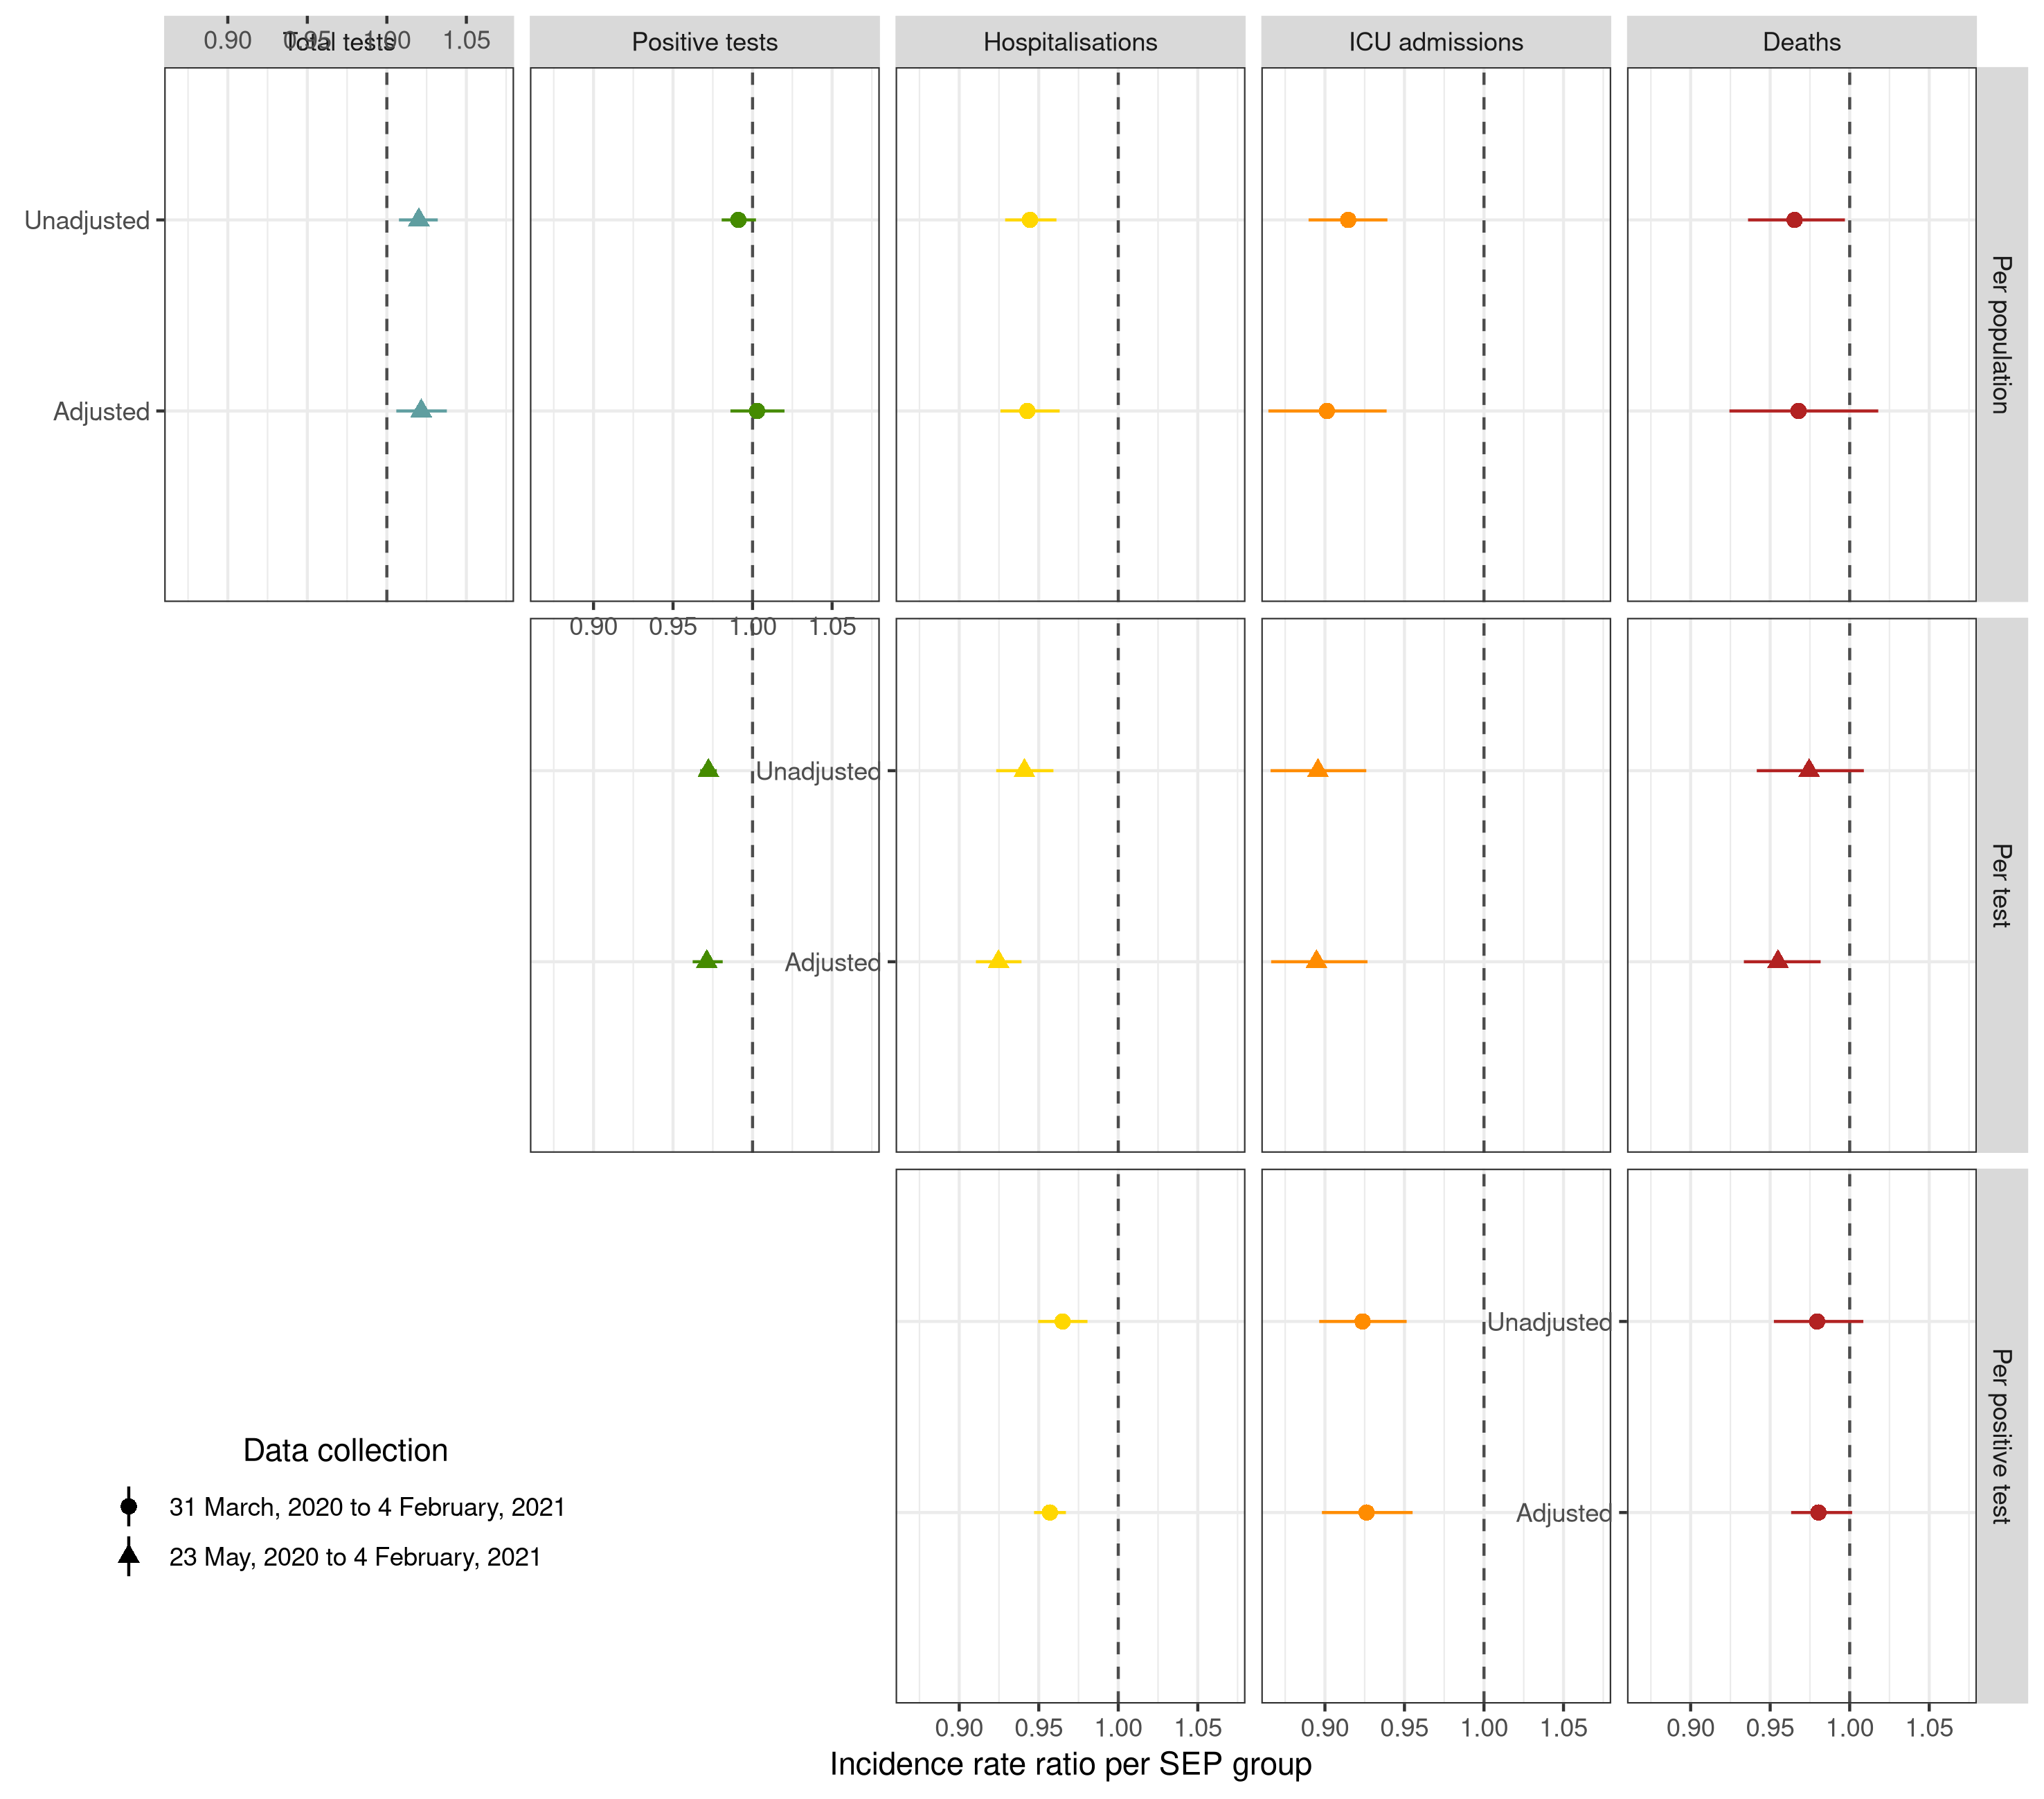
\includegraphics[width=\linewidth]{suppfigure_adj_covariates.png}
		\caption{Incidence rate ratios (95\% credible interval) for the association between age, sex and epidemic wave and five outcomes related to SARS-CoV-2 surveillance and care: total tests, positive tests, hospitalisations, intensive care unit (ICU) admissions and deaths. The reference group for age is 40-49 (squares) for total tests, positive tests and hospitalisations. Because of the small number of events in younger groups, we pooled together age groups 0 to 49 for ICU admissions and deaths, and used this larger group as reference. The reference group is males and the first epidemic wave. The models are also adjusted for canton and SEP decile.}
		\label{fig:adj-cov}
	\end{figure}


Figure \ref{fig:adj-canton} shows the association between canton and each outcome. 
As the canton effect was formulated using a random intercept (and a random slope, see below), the interpretation does not rely upon a reference group but to the overall average.
For instance, there has been around 3 times more deaths per population in canton Ticino (TI) compared to average.
The geographic heterogeneity can be assessed by comparing the spread of cantons, or by looking at the inter-cantonal variance (Figure \ref{fig:het-canton}).
This inter-cantonal variance corresponds to $\sigma_{\alpha}^2$ in equation \ref{eq:m3b}.
For instance, there is more inter-cantonal variation in the number of deaths per population (more affected by the total size of the epidemic) than in the number of deaths per positive test (more affected by the quality of care).

Tables \ref{tab:cov-age}, \ref{tab:cov-sex} and \ref{tab:cov-wave} present the same estimates in tabular form.

\begin{figure}[H]
	\centering
	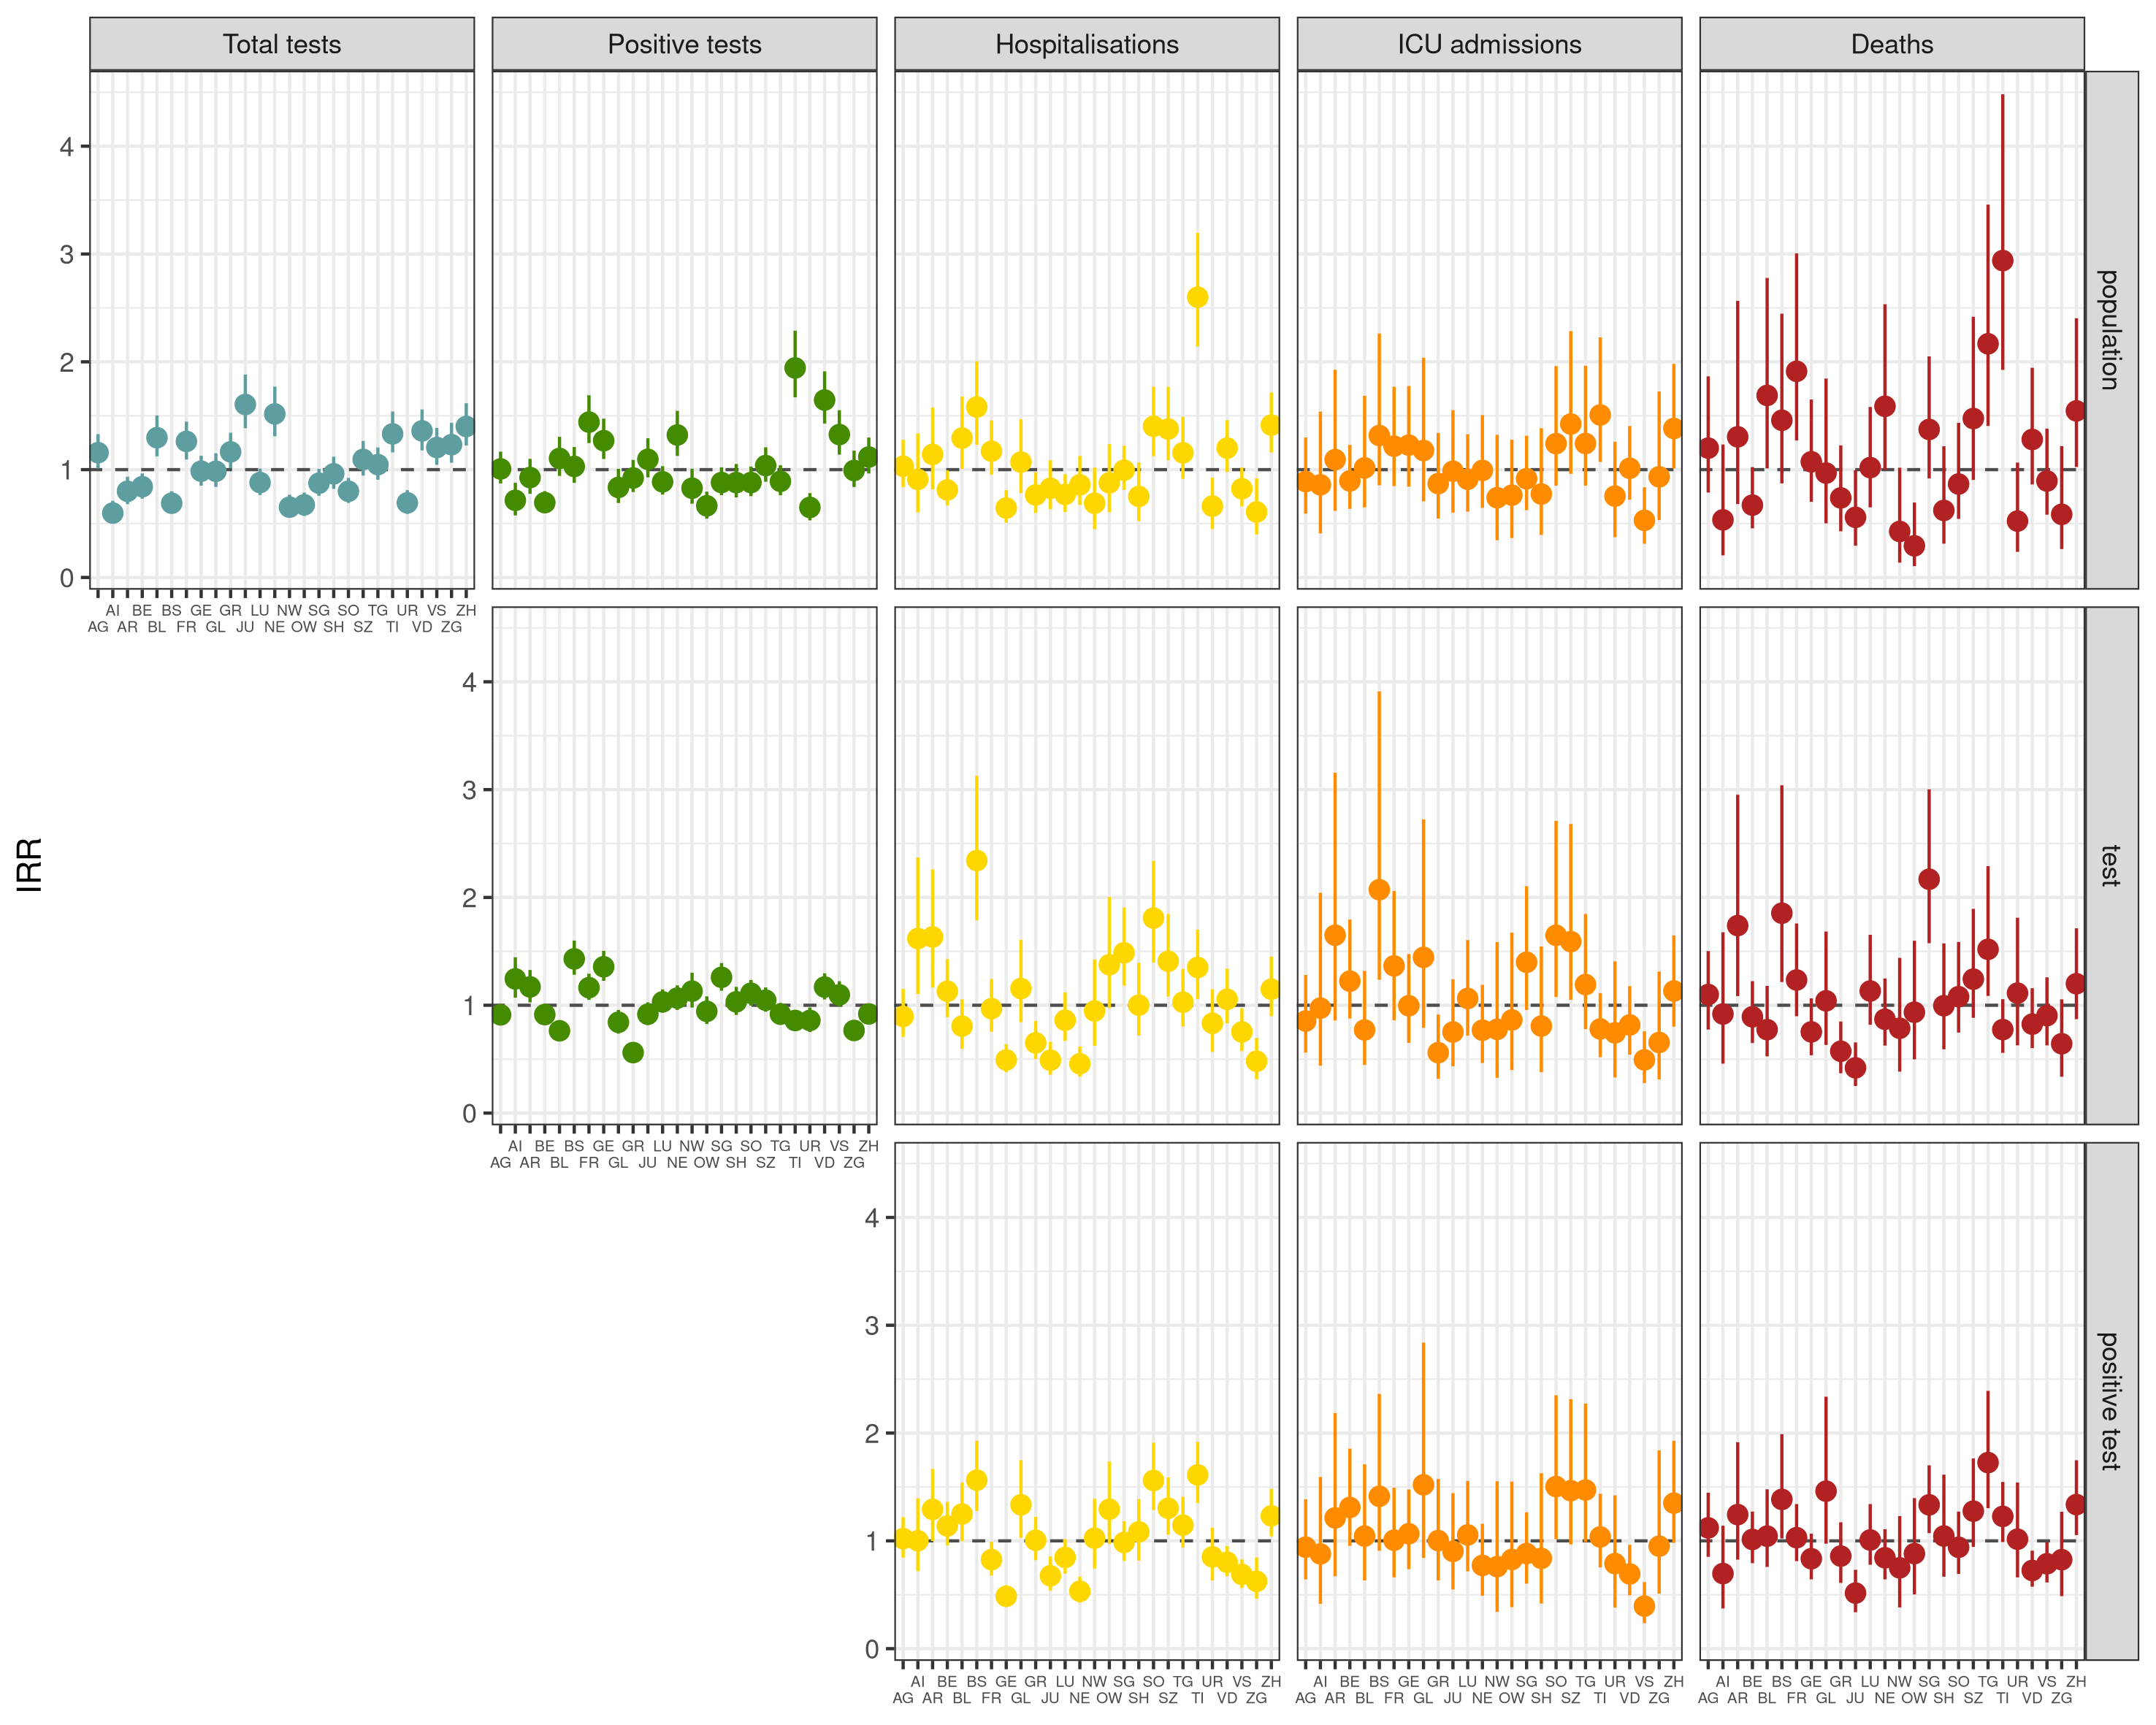
\includegraphics[width=\linewidth]{suppfigure_adj_canton.png}
	\caption{Incidence rate ratios (95\% credible interval) for the association between each canton and five outcomes related to SARS-CoV-2 surveillance and care: total tests, positive tests, hospitalisations, intensive care unit (ICU) admissions and deaths.
	As this is implemented as a random intercept, there is no reference groups and the incidence rate ratios must be interpreted relatively to the overall average. The models are also adjusted for age, sex, epidemic wave and SEP decile.}
	\label{fig:adj-canton}
\end{figure}


\begin{figure}[H]
	\centering
	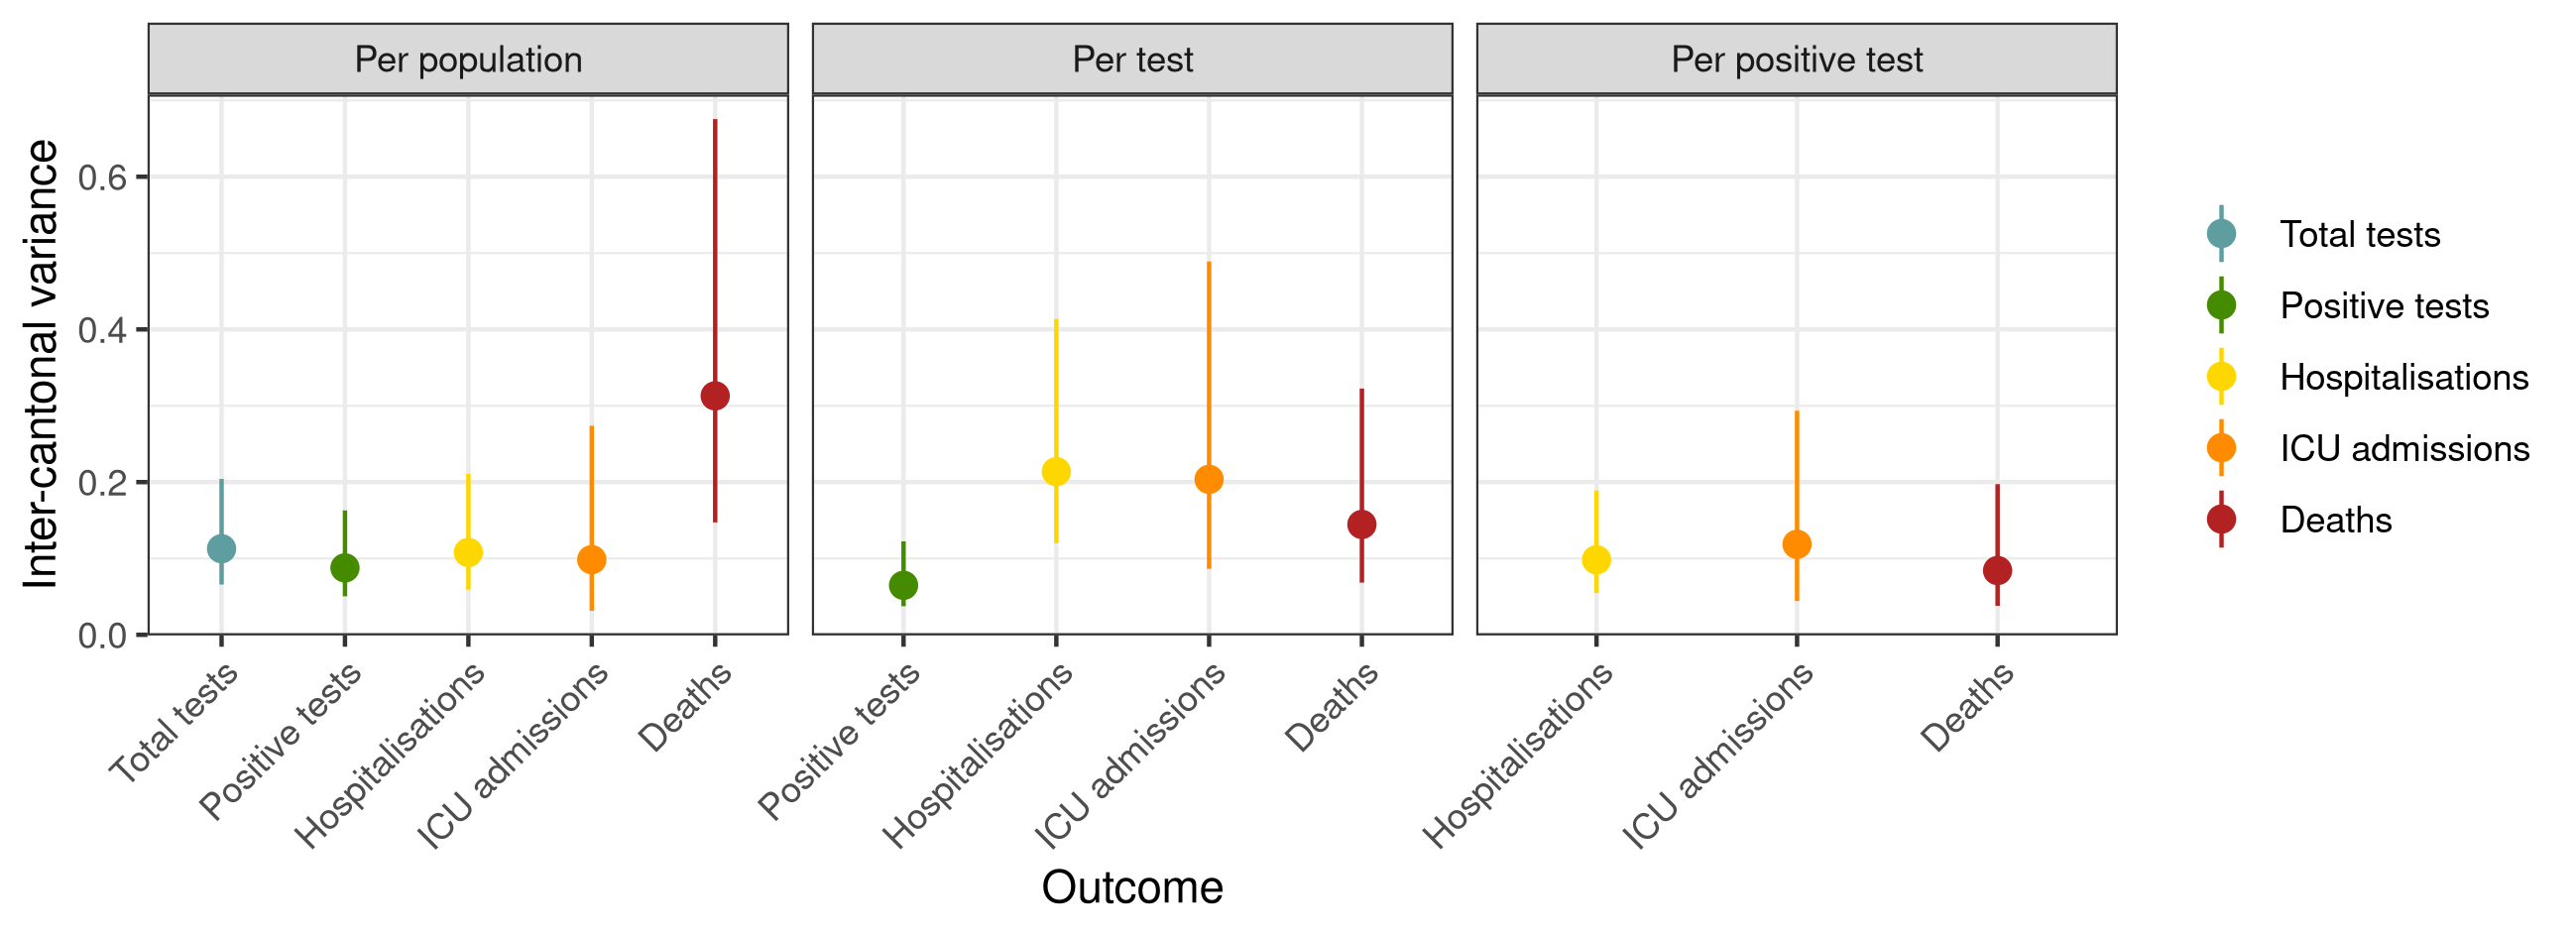
\includegraphics[width=\linewidth]{suppfigure_het_canton.png}
	\caption{Inter-cantonal variance (95\% credible interval) of the association between each canton and five outcomes related to SARS-CoV-2 surveillance and care: total tests, positive tests, hospitalisations, intensive care unit (ICU) admissions and deaths.}
	\label{fig:het-canton}
\end{figure}

	
	\subsection{Interaction analysis}
	\label{sec:int}
	
	We now consider two-way interactions between each covariate (age, sex, epidemic wave and canton) and SEP, to assess whether the association between SEP and each outcome is modified by these other factors.
	We start with the canton, as the interaction with canton is already included in model 2 (the adjusted model that is used for the main results) as a ``random slope'' (see equations \ref{eq:m3} and \ref{eq:m3b}).
	
	Figure \ref{fig:slope-canton} shows estimates of the association between SEP and each outcome (IRR per SEP decile) in each canton. 
	Going back to equation \ref{eq:m3b}, these correspond to $\exp(\beta_j)$ for each canton $j$, computed from the average effect of SEP $\mu_{\beta}$, the inter-cantonal variance $\sigma_{\beta}^2$ and from the deviation in each canton (the random slope) $b_j$.
	We observe large deviations from average in some cantons, for instance in Geneva (GE) for total tests per population. 
	This can be interpreted as: the positive association between SEP and total tests per population is even steeper in Geneva compared to average.
	More generally, we observe a reduction in cantonal heterogeneity as we move from the population denominator to the test or positive test.
	This can be quantified by the estimate of inter-cantonal variance (Figure \ref{fig:het-slope-canton}).
	
	\begin{figure}[H]
		\centering
		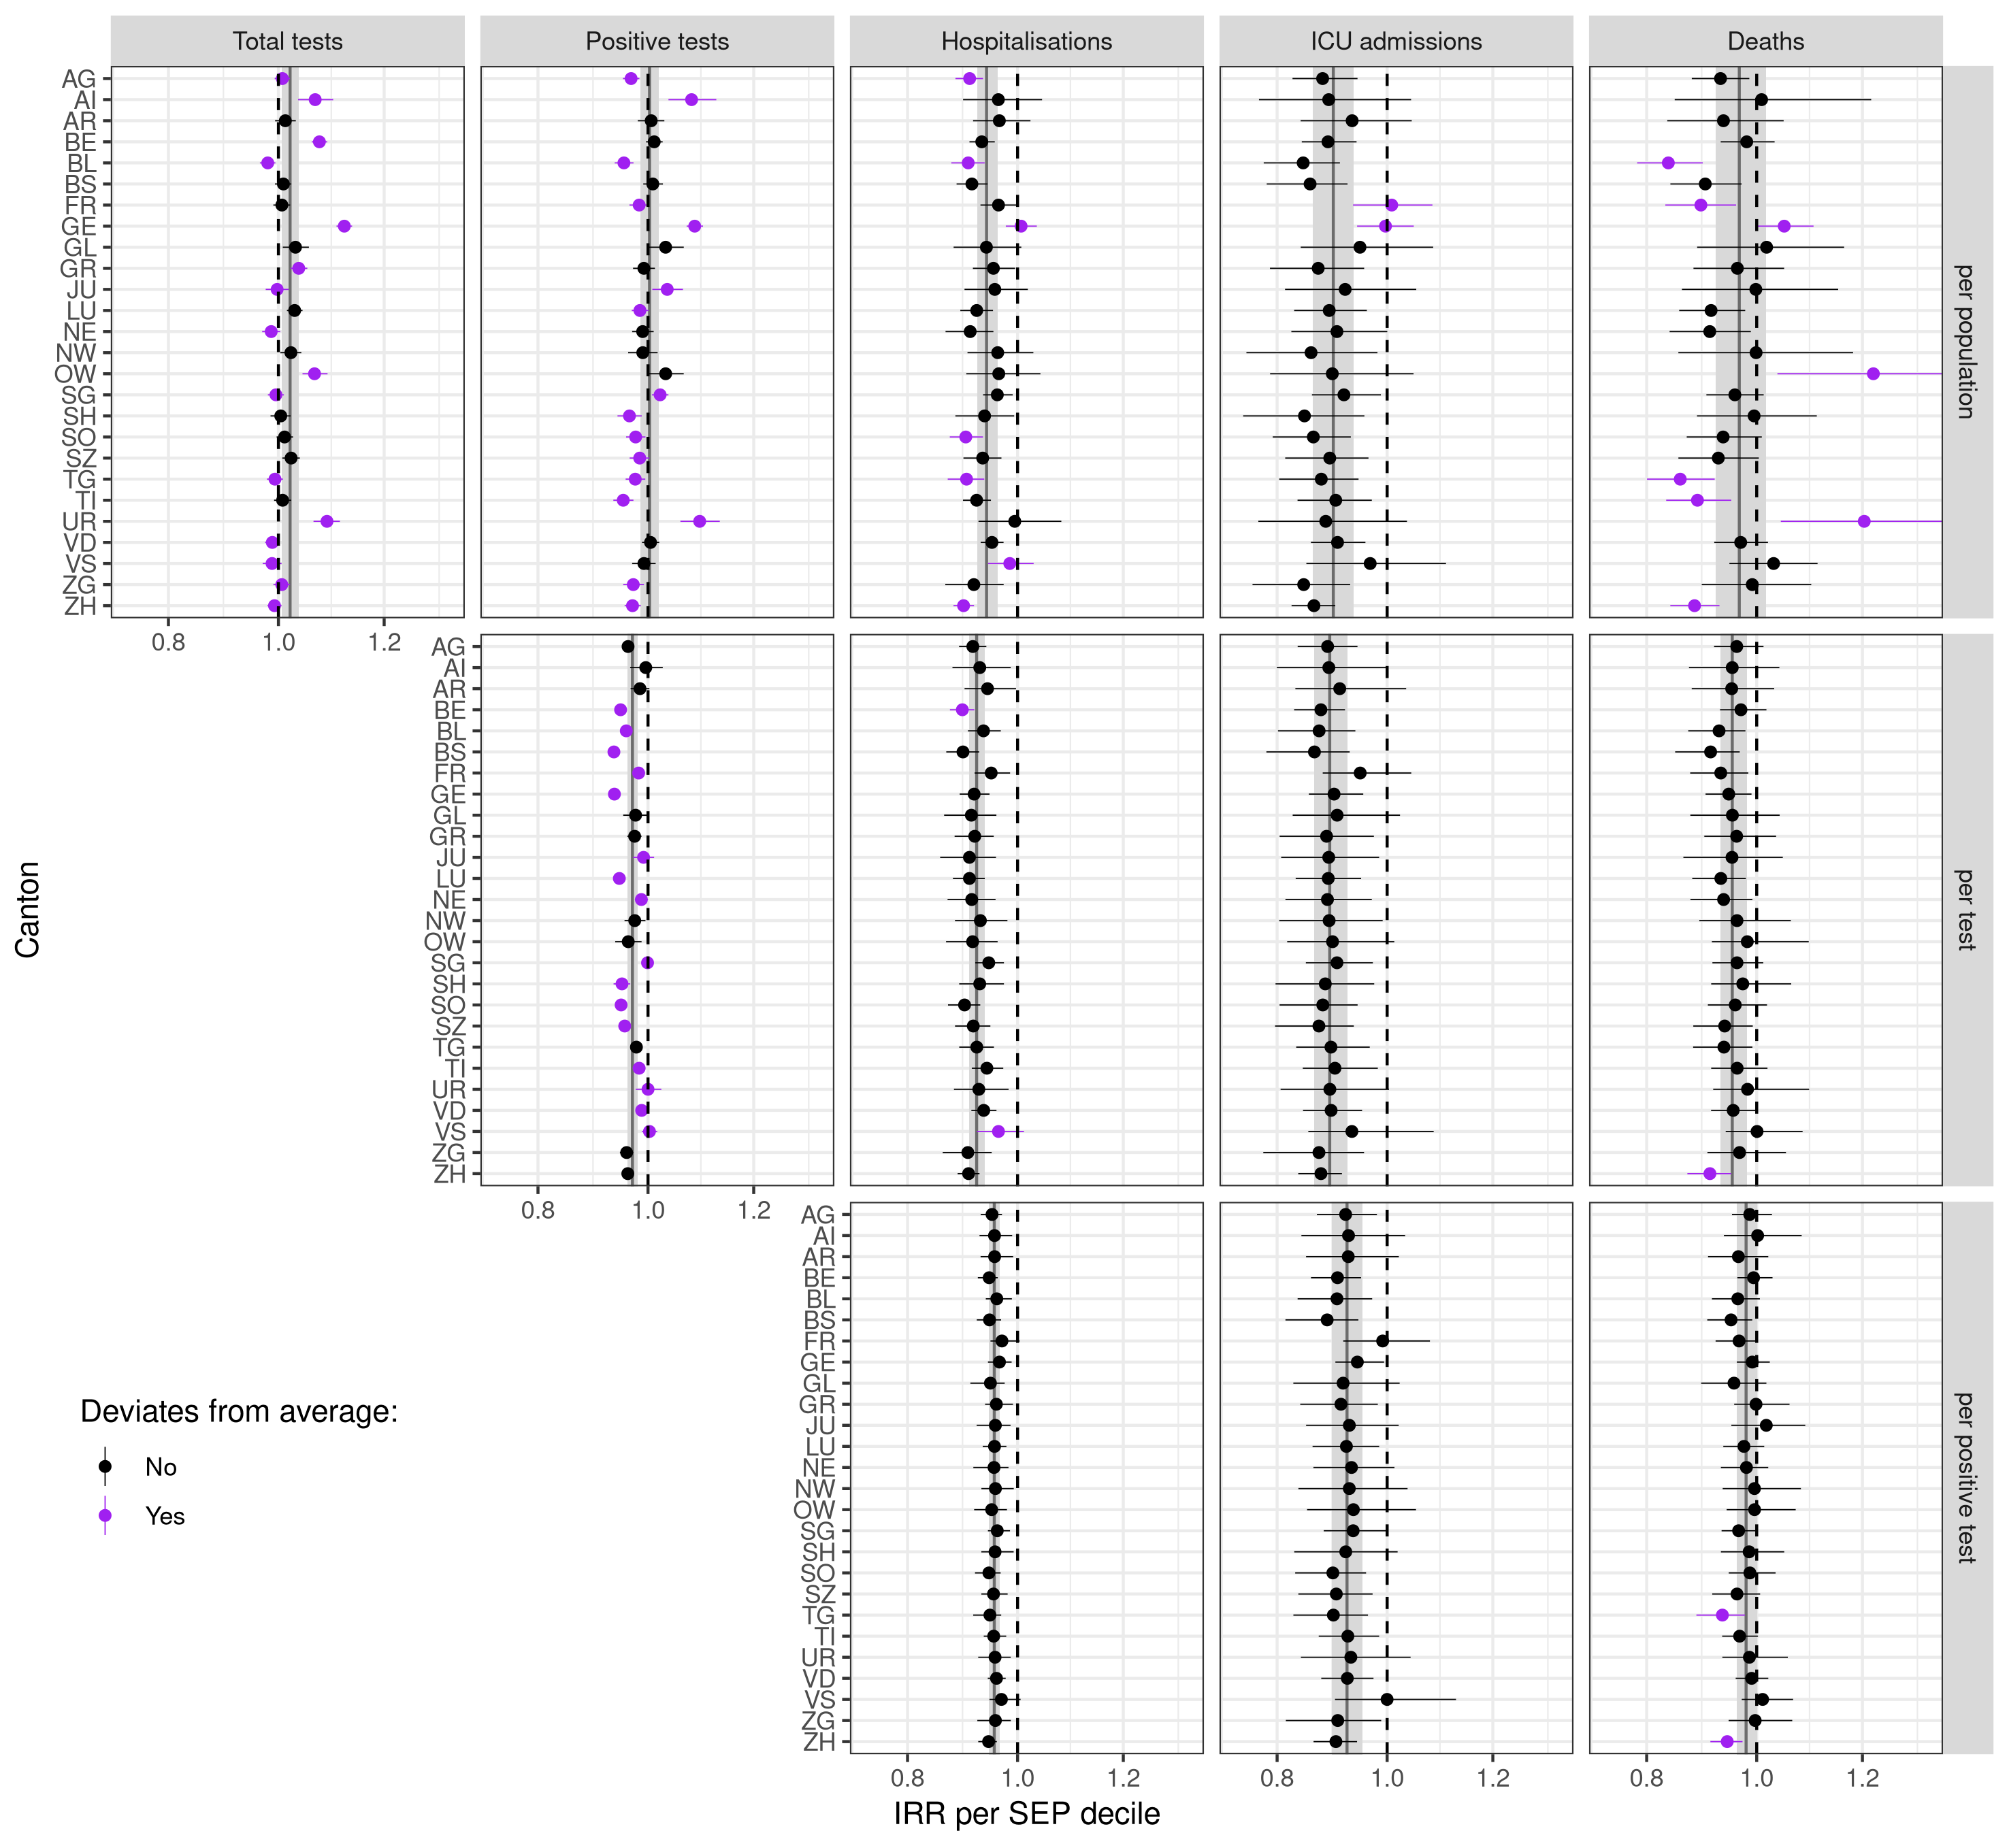
\includegraphics[width=\linewidth]{suppfigure_irr_by_canton.png}
		\caption{Incidence rate ratios (95\% credible interval) for the association between socio-economic position (SEP) and five outcomes, \textit{separately in each canton}. Deviation from average (highlighted in purple) is defined as the 95\% credible interval in the canton not including the overall average (shown by the full line and shaded area). Credible intervals are truncated at 1.3 for visibility, exact numbers are available in Table \ref{tab:slope-canton}.}
		\label{fig:slope-canton}
	\end{figure}

	\begin{figure}[H]
	\centering
	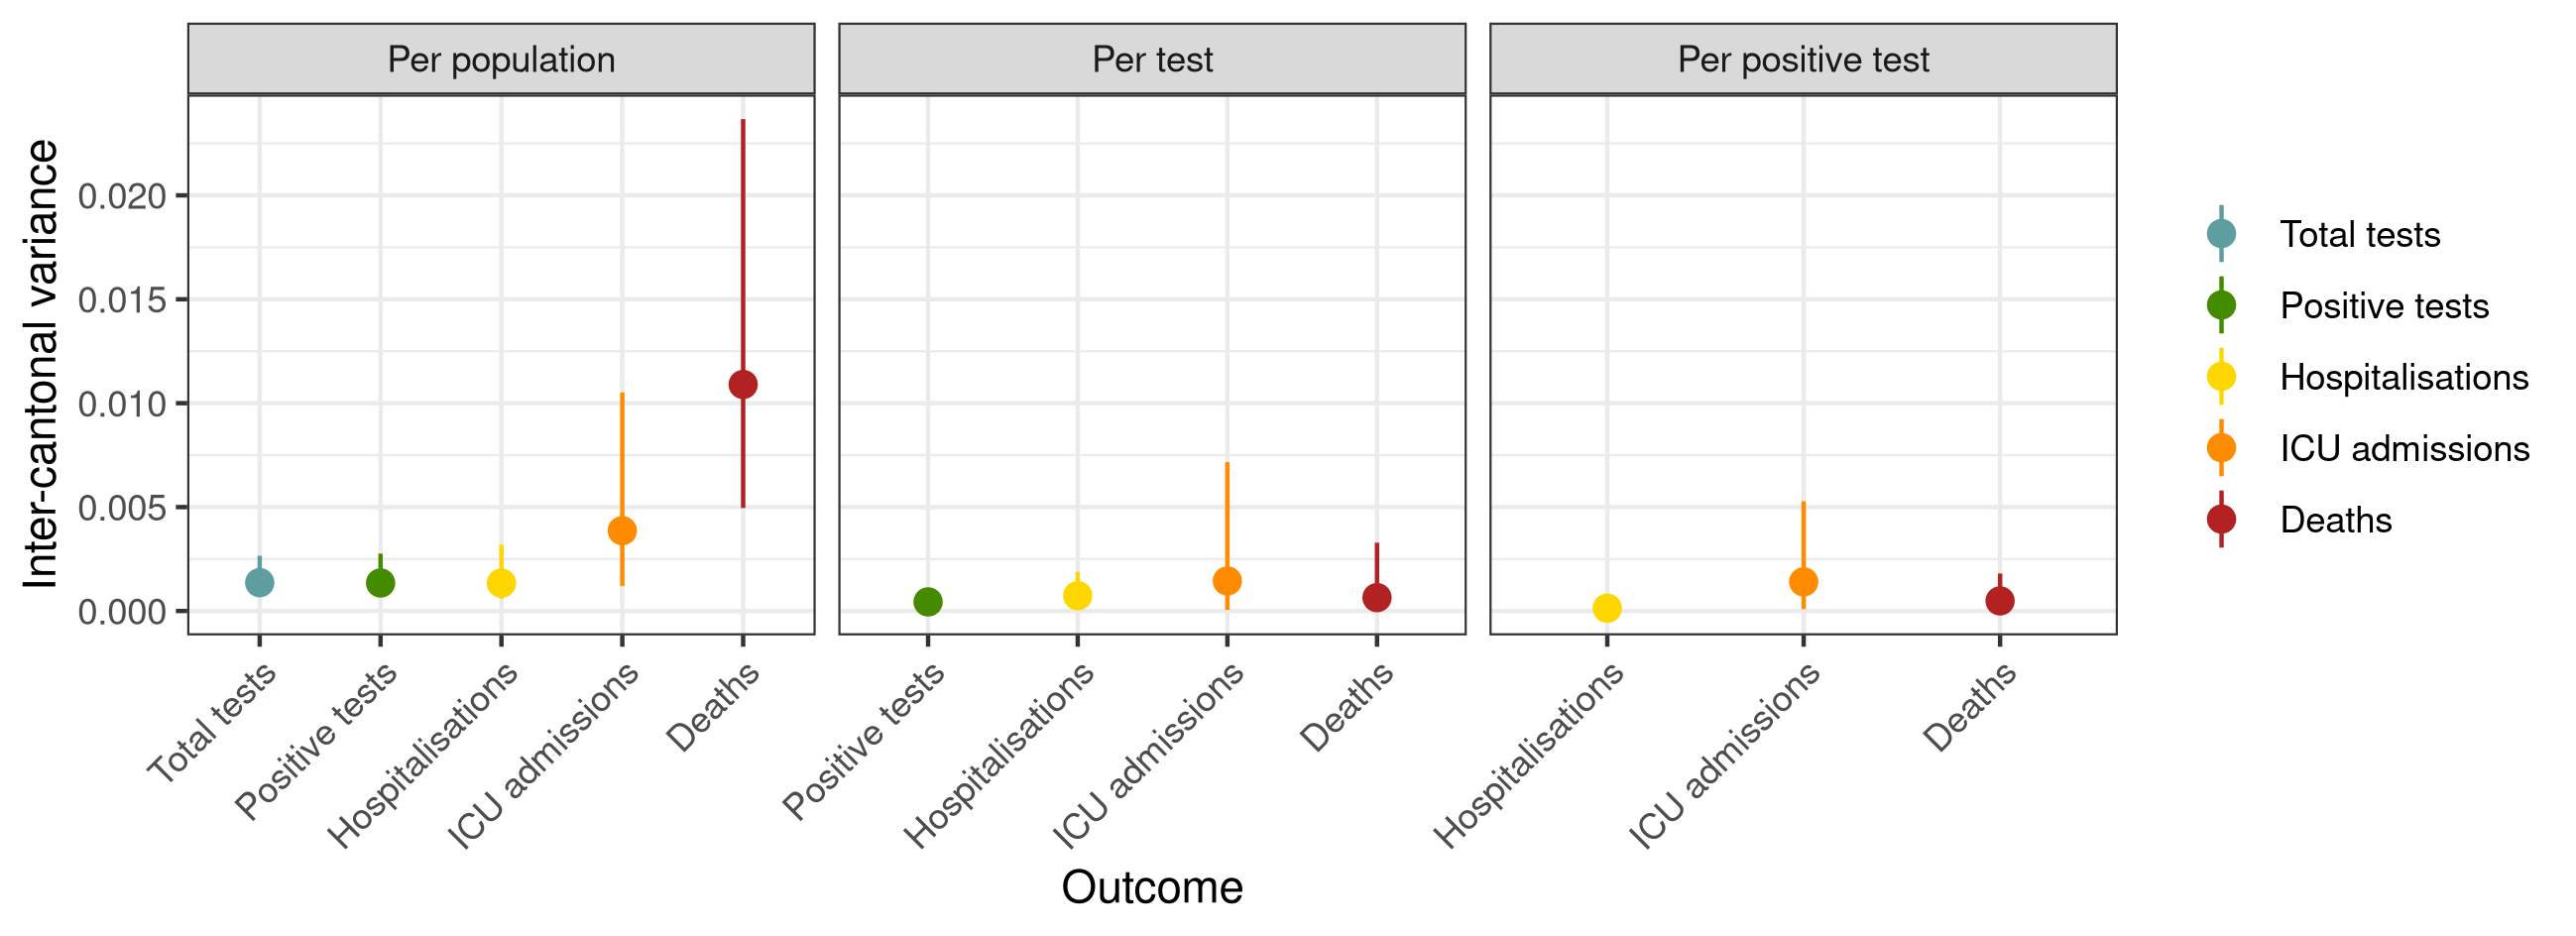
\includegraphics[width=\linewidth]{suppfigure_het_slope_canton.png}
	\caption{Inter-cantonal variance (95\% credible interval) of the association between SEP and five outcomes related to SARS-CoV-2 surveillance and care, \textit{separately in each canton}.}
	\label{fig:het-slope-canton}
\end{figure}
	
	Figure \ref{fig:slope-cov} shows estimates of the association between SEP and each outcome (IRR per SEP decile) by age, sex and epidemic wave. 
	These estimates come from  model 3, including all two-way interactions.
	We observe for all combinations of outcome and denominator that the association between SEP and the outcome decreases in older age groups.
	This observation is especially meaningful for deaths per population, per test and per positive tests, because a large proportion of deaths (71\%) occur in the 80+ age group, where the association between SEP and mortality is the weakest (IRR close to 1).
	The fact that the association between SEP and mortality appears strongly in other age groups (IRRs consistently below 1) suggests that the absence of association found on average in the population is misleading, and that SEP and mortality are actually associated.
	We don't find evidence that the association between SEP and each outcomes varies systematically according to sex or epidemic period.
	One exception is positive tests per population, where we observe a diminution of the IRR between the first and second epidemic wave. 
	This point is further developed in section \ref{sec:period}.
	Estimates obtained with tests as a denominator show large uncertainty during the first wave, because total tests were only available from 23 May 2020 onwards, meaning that the estimate for the first wave (before 8 June) is based on only 2 weeks of data. 
	These should be interpreted with caution.
	
	
	\begin{figure}[H]
		\centering
		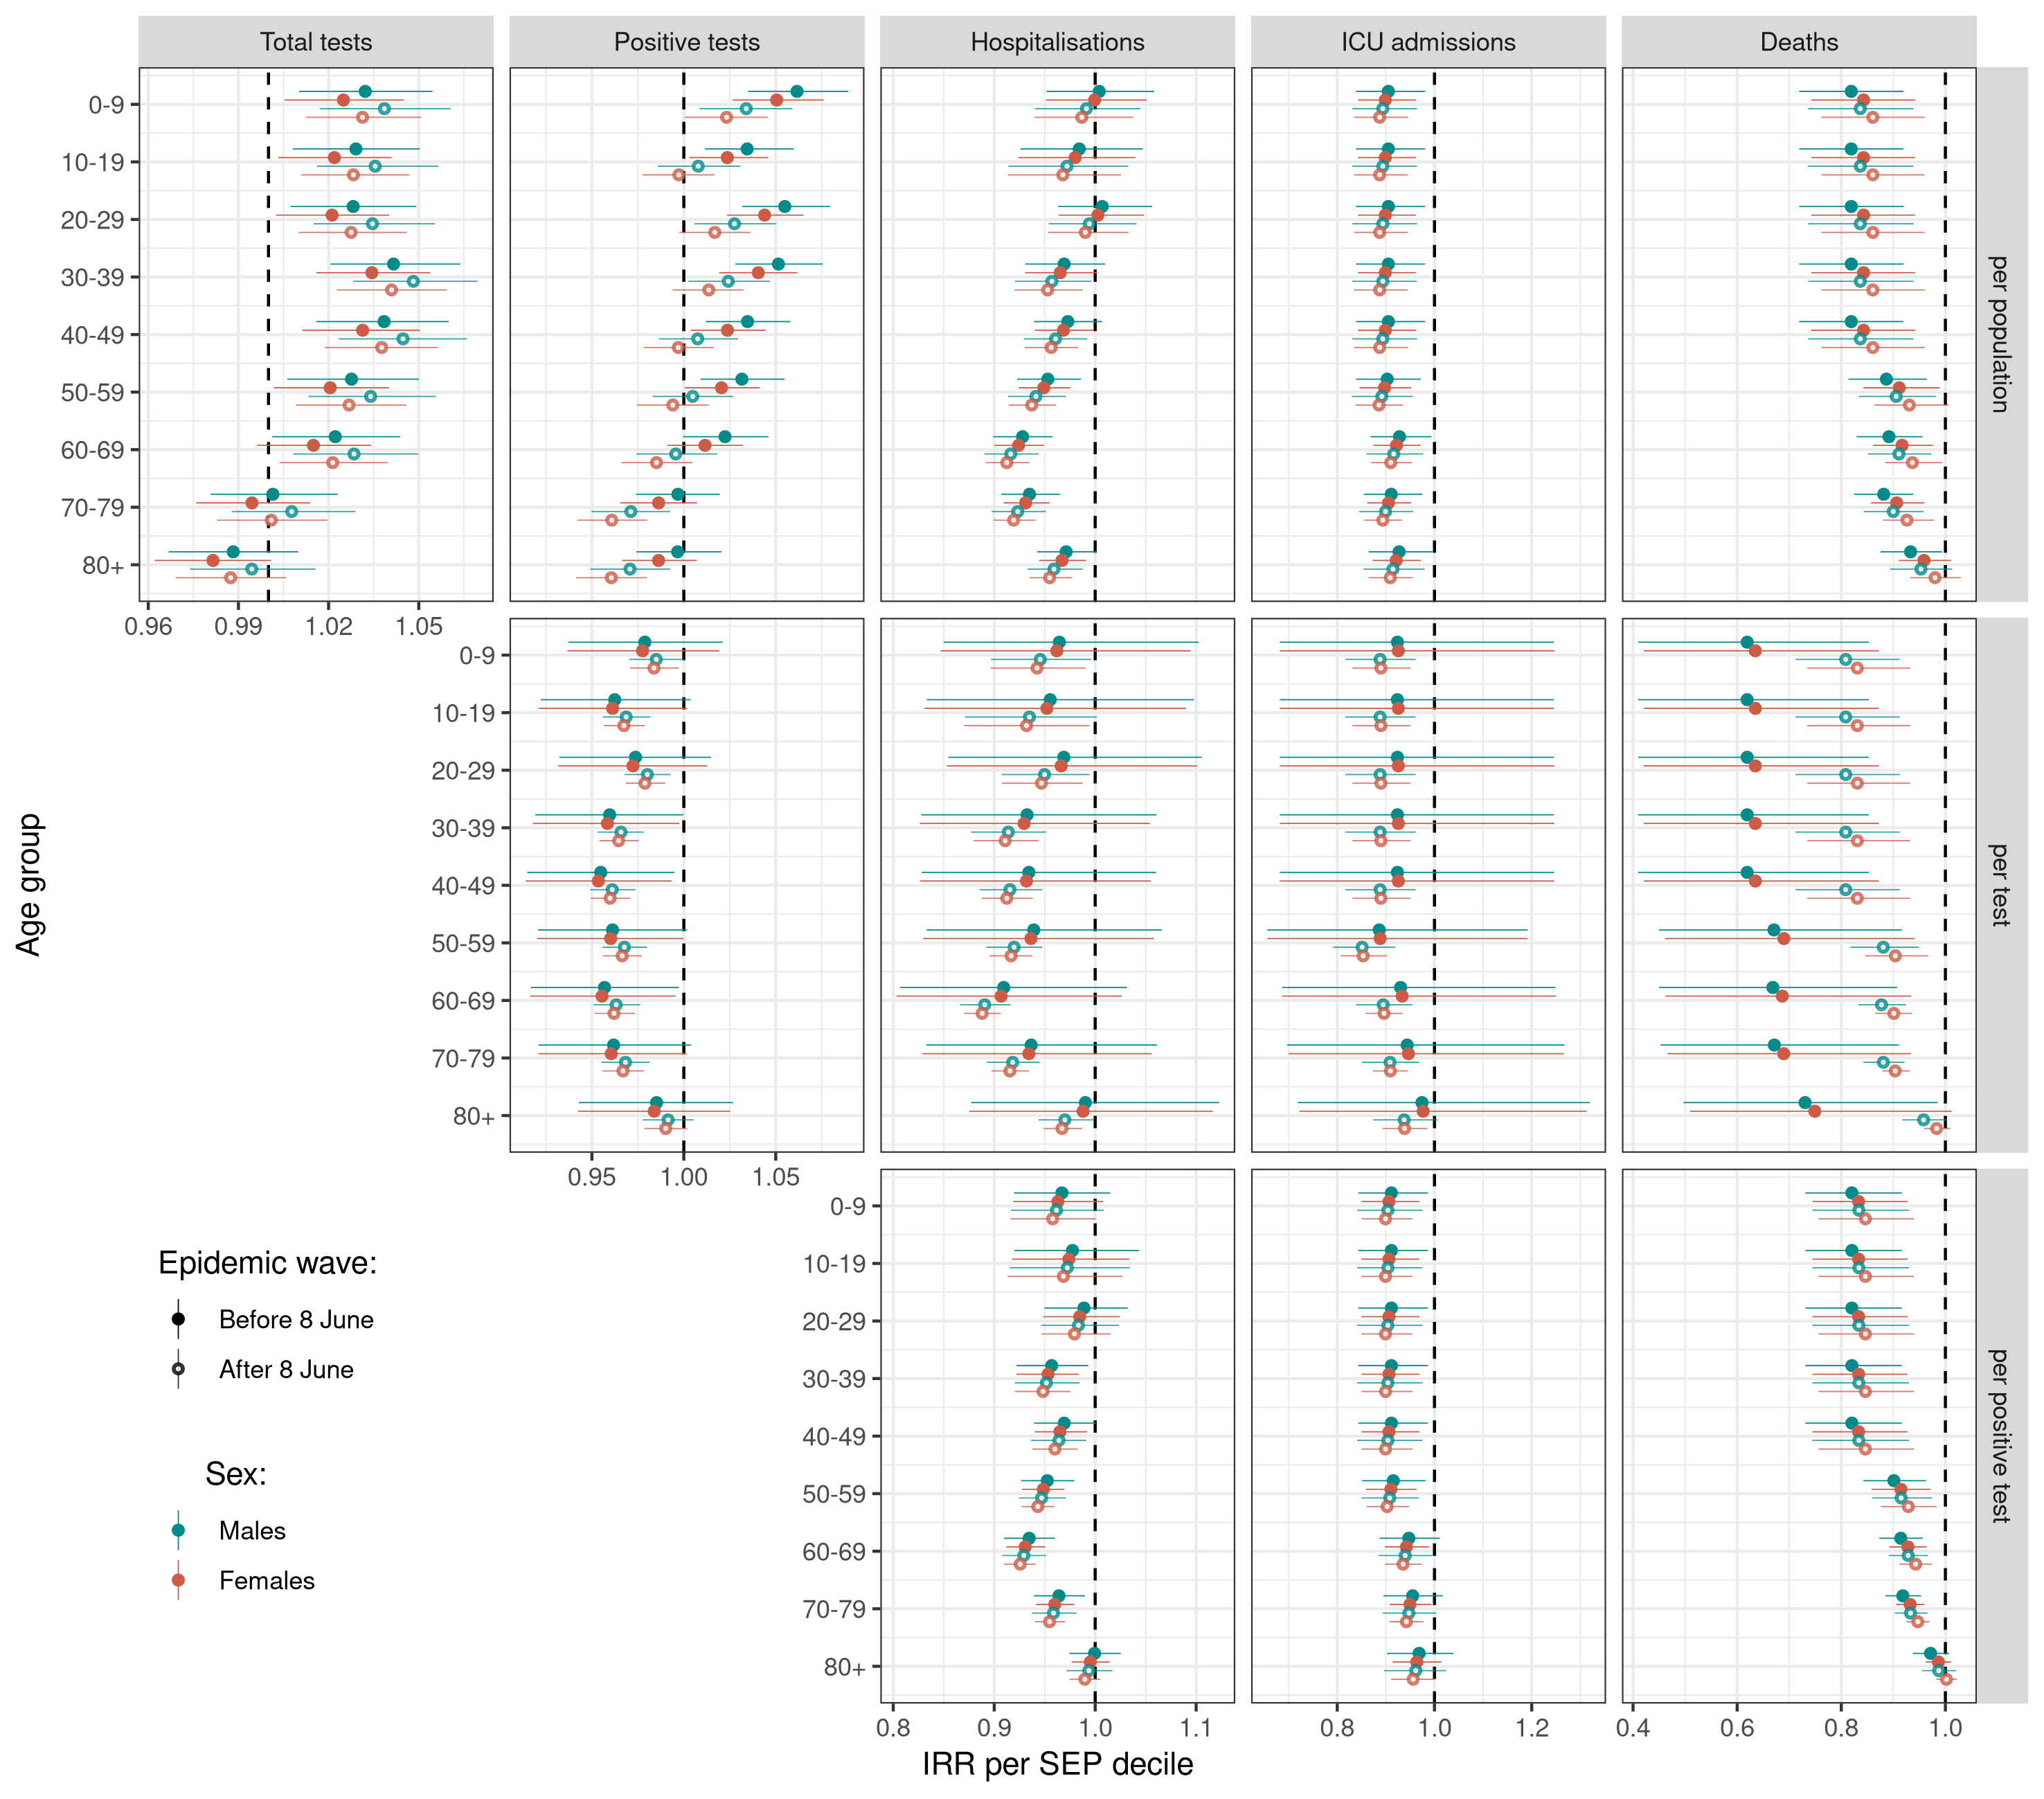
\includegraphics[width=\linewidth]{suppfigure_irr_by_interactions.png}
		\caption{Incidence rate ratios (95\% credible interval) for the association between socio-economic position (SEP) and five outcomes, \textit{separately in each combination of age group, sex and epidemic wave}. }
		\label{fig:slope-cov}
	\end{figure}
	
	\section{Sensitivity analyses}
	\subsection{Stratification by period}
	\label{sec:period}
	
	The issue with model fit for positive tests per population explained in section \ref{sec:fit}, together with the interaction between SEP and epidemic wave spotted in section \ref{sec:int} led us to further explore the effect of epidemic wave on the results.
	To do that, we repeated the analyses after stratifying by epidemic wave (before/after 8 June, 2020).
	Figure \ref{fig:fit_strat} shows the model fit after applying the stratification. We observe a clear improvement of the model fit to positive tests per population (i.e., test positivity) and deduce the cause of the issue.
	The association between SEP and test positivity changed from being positive (IRR per SEP decile: 1.02 [95\%CrI: 1.01-1.03]) during the first wave to slightly negative (IRR per SEP decile: 0.99 [95\%CrI: 0.98-0.99]) during the second wave.
	In accordance with the results from the interaction analyses, we didn't find other differences between epidemic waves (Figure \ref{fig:est_strat}).
	We also don't see clear differences in the effect of other covariates (Figure \ref{fig:cov_strat}).
	
%	Figure S5 (model fit by period) 

	\begin{figure}[H]
	\centering
	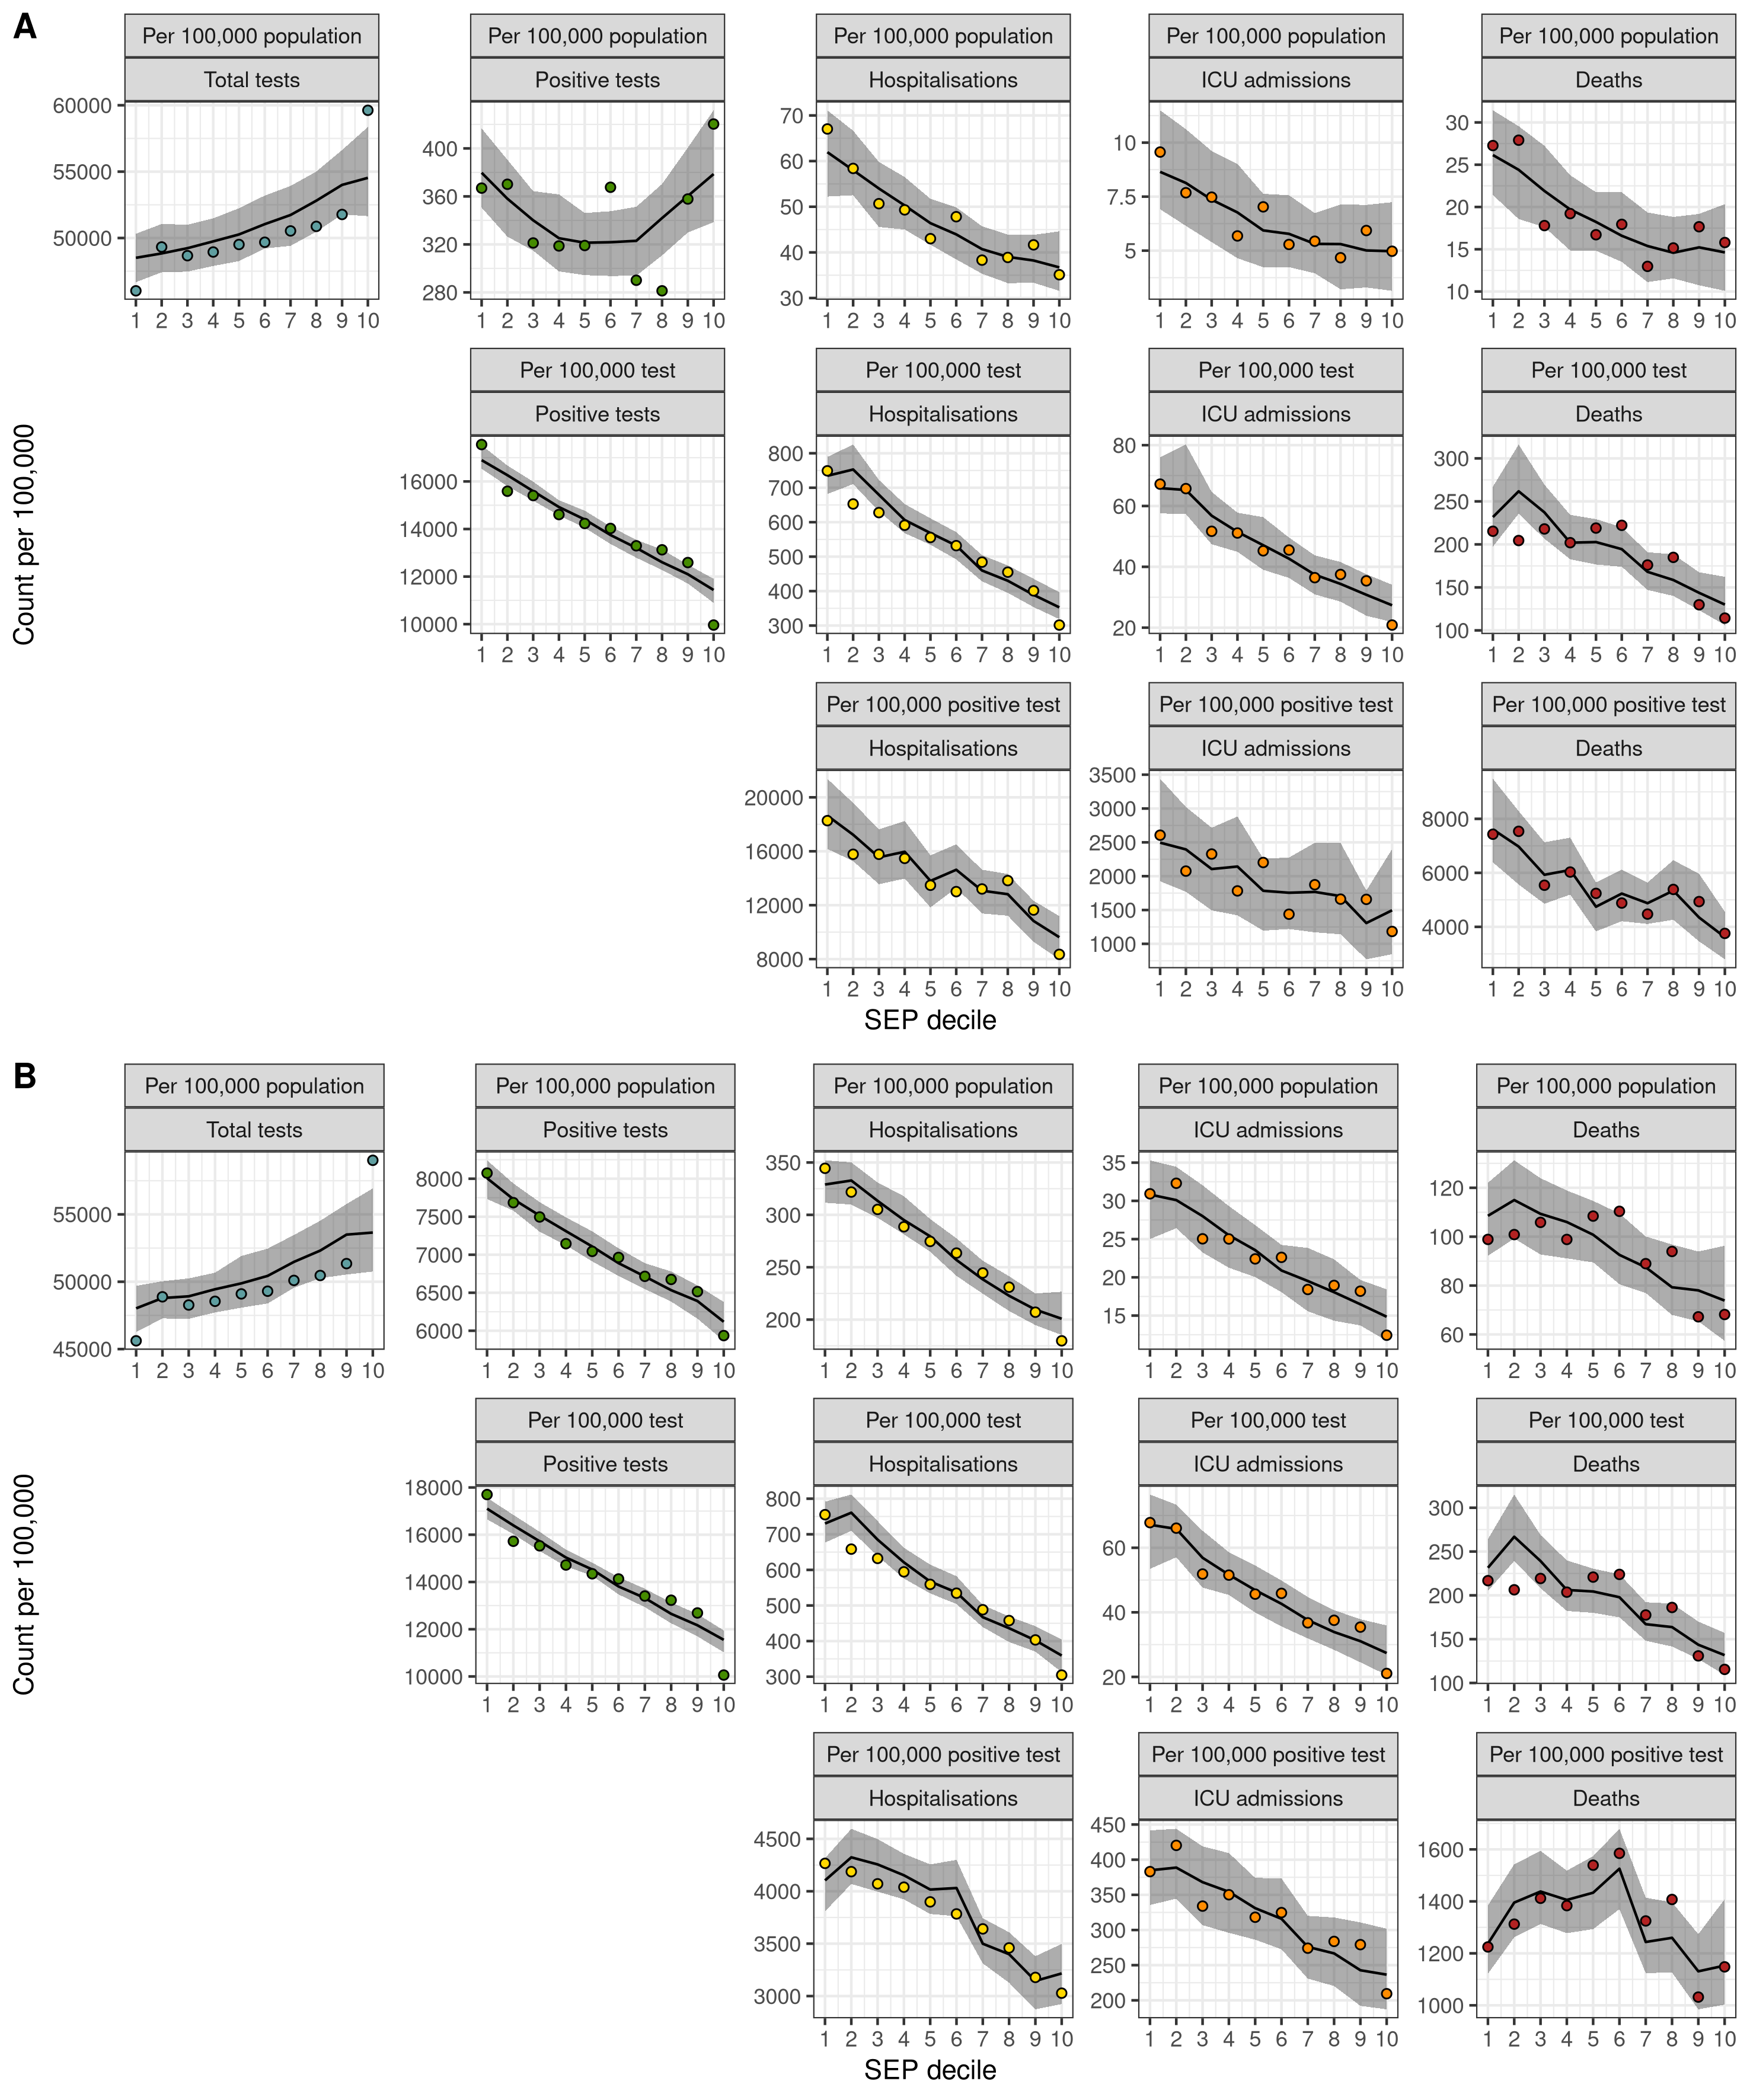
\includegraphics[width=\linewidth]{suppfigure_model_fit_stratified_by_period_8june.png}
	\caption{Fit of the models adjusted for age, sex, epidemic wave and canton by epidemic wave (panel A: 1st wave until 8 June, 2020; panel B: 2nd wave from 8 June, 2020). Circles show data points, the line and shaded area show the corresponding model prediction (median and 95\% prediction interval).}
	\label{fig:fit_strat}
\end{figure}

% Figure S6 (model estimates by period)

	\begin{figure}[H]
	\centering
	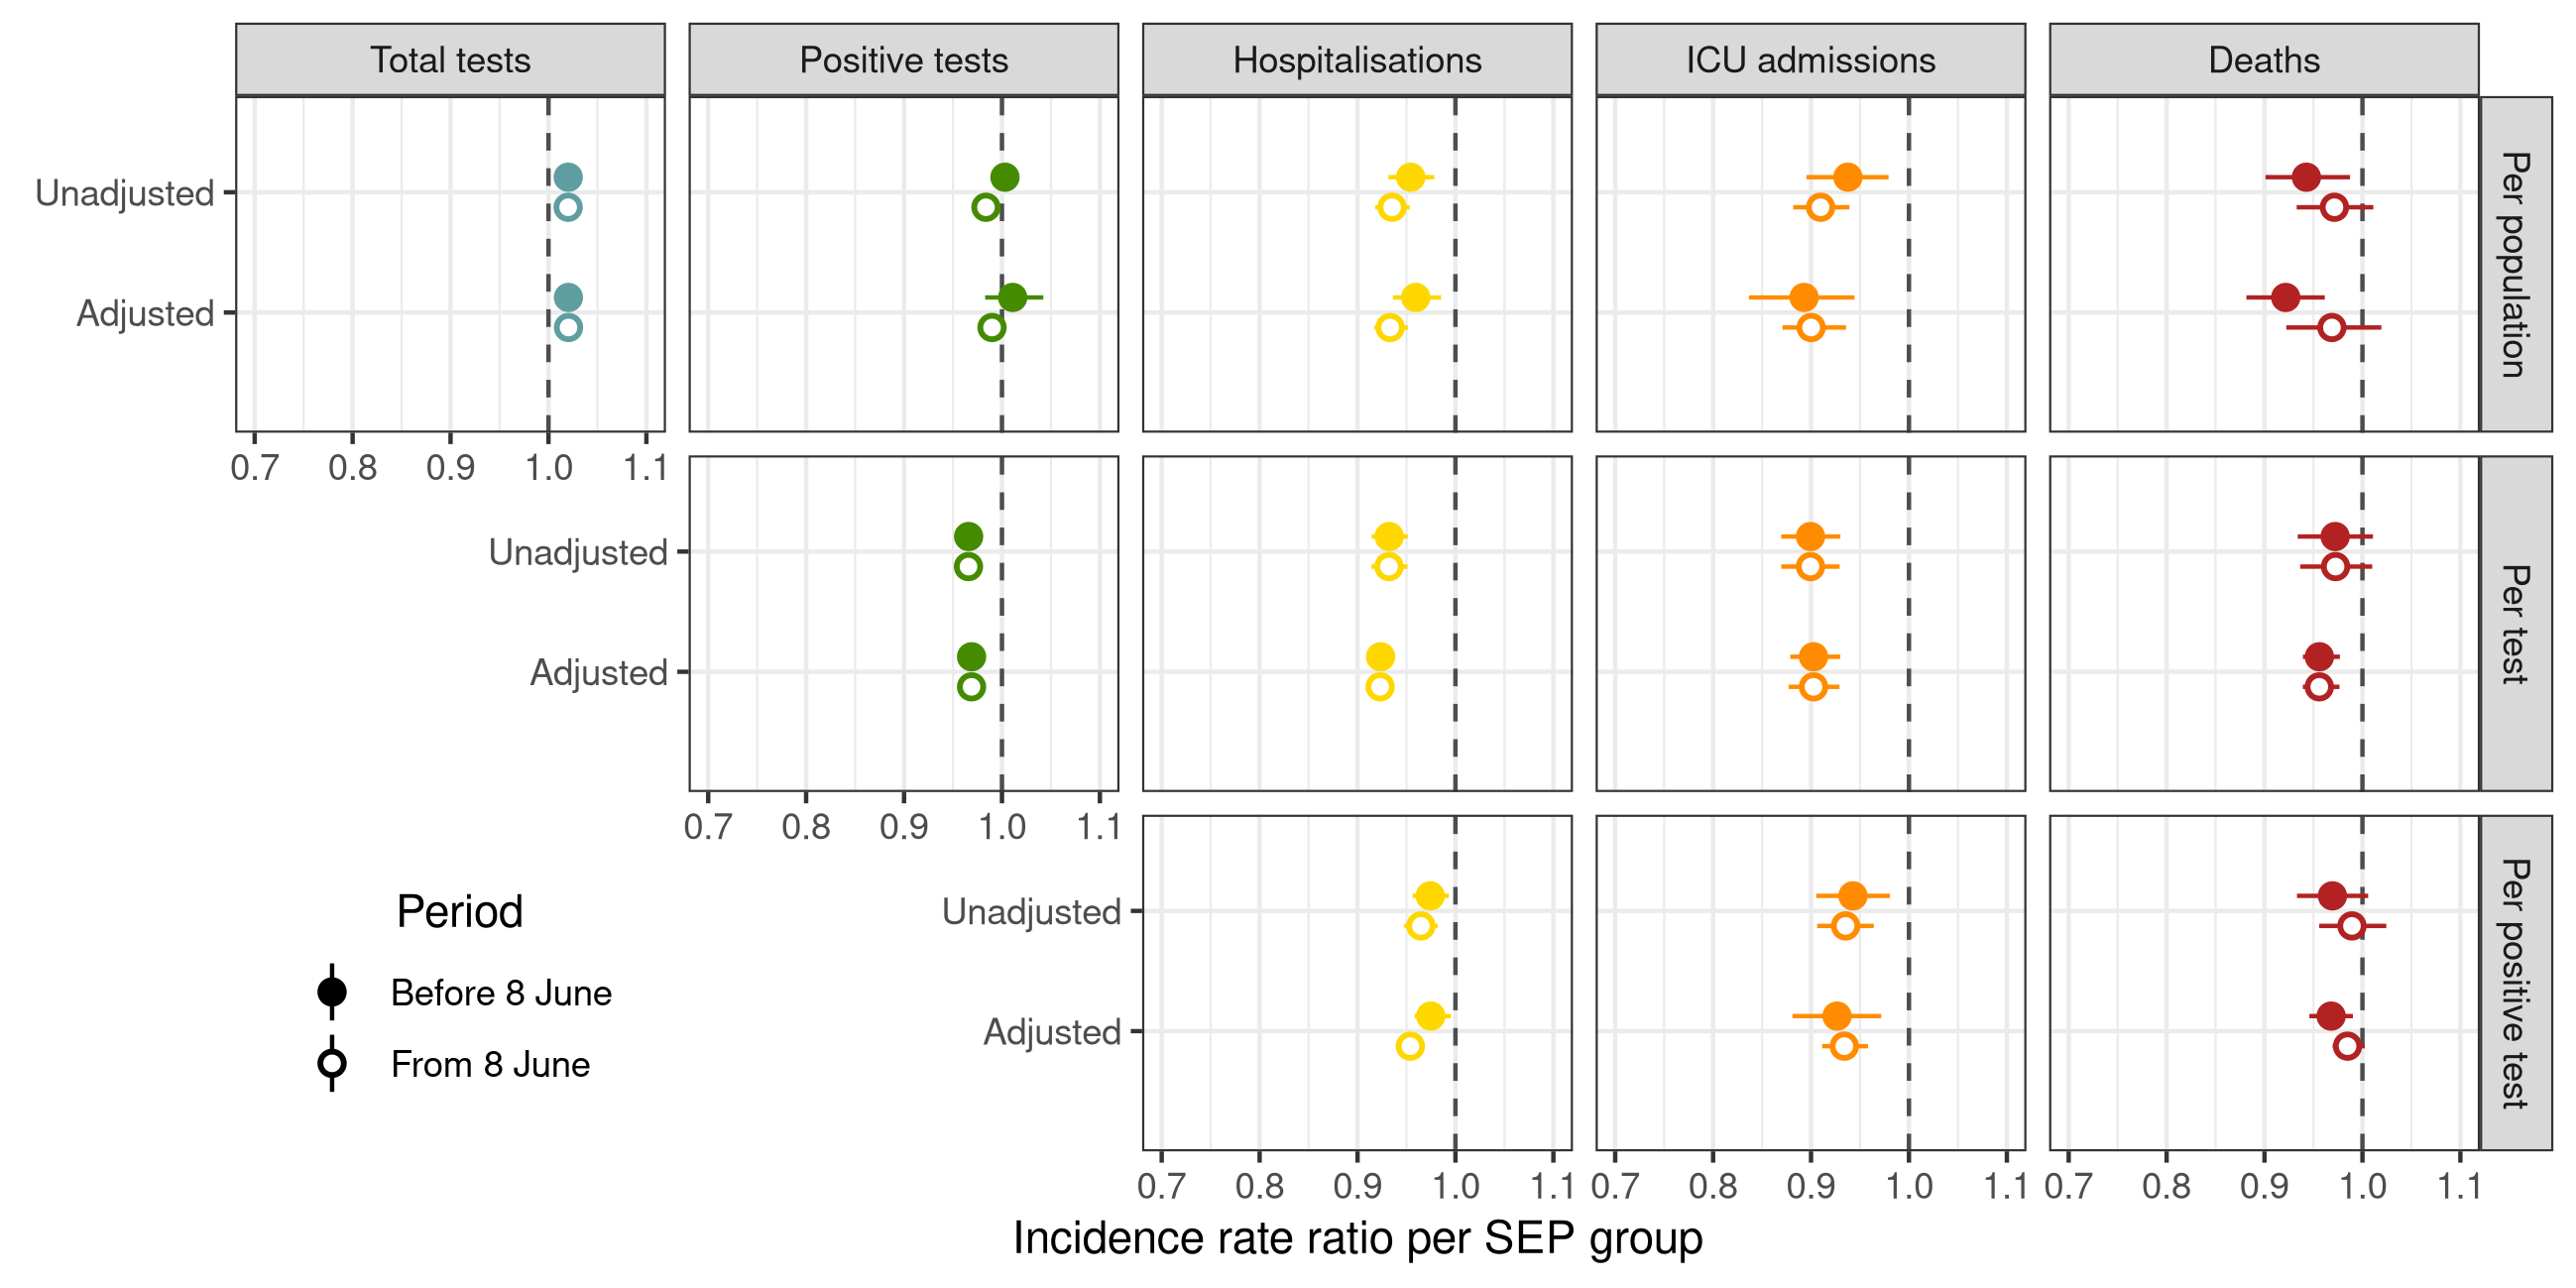
\includegraphics[width=\linewidth]{suppfigure_model_estimates_strat_by_period_8june.png}
	\caption{Estimates of incidence rate ratios per decile of SEP stratified by epidemic wave.}
	\label{fig:est_strat}
\end{figure}
	
		\begin{figure}[H]
		\centering
		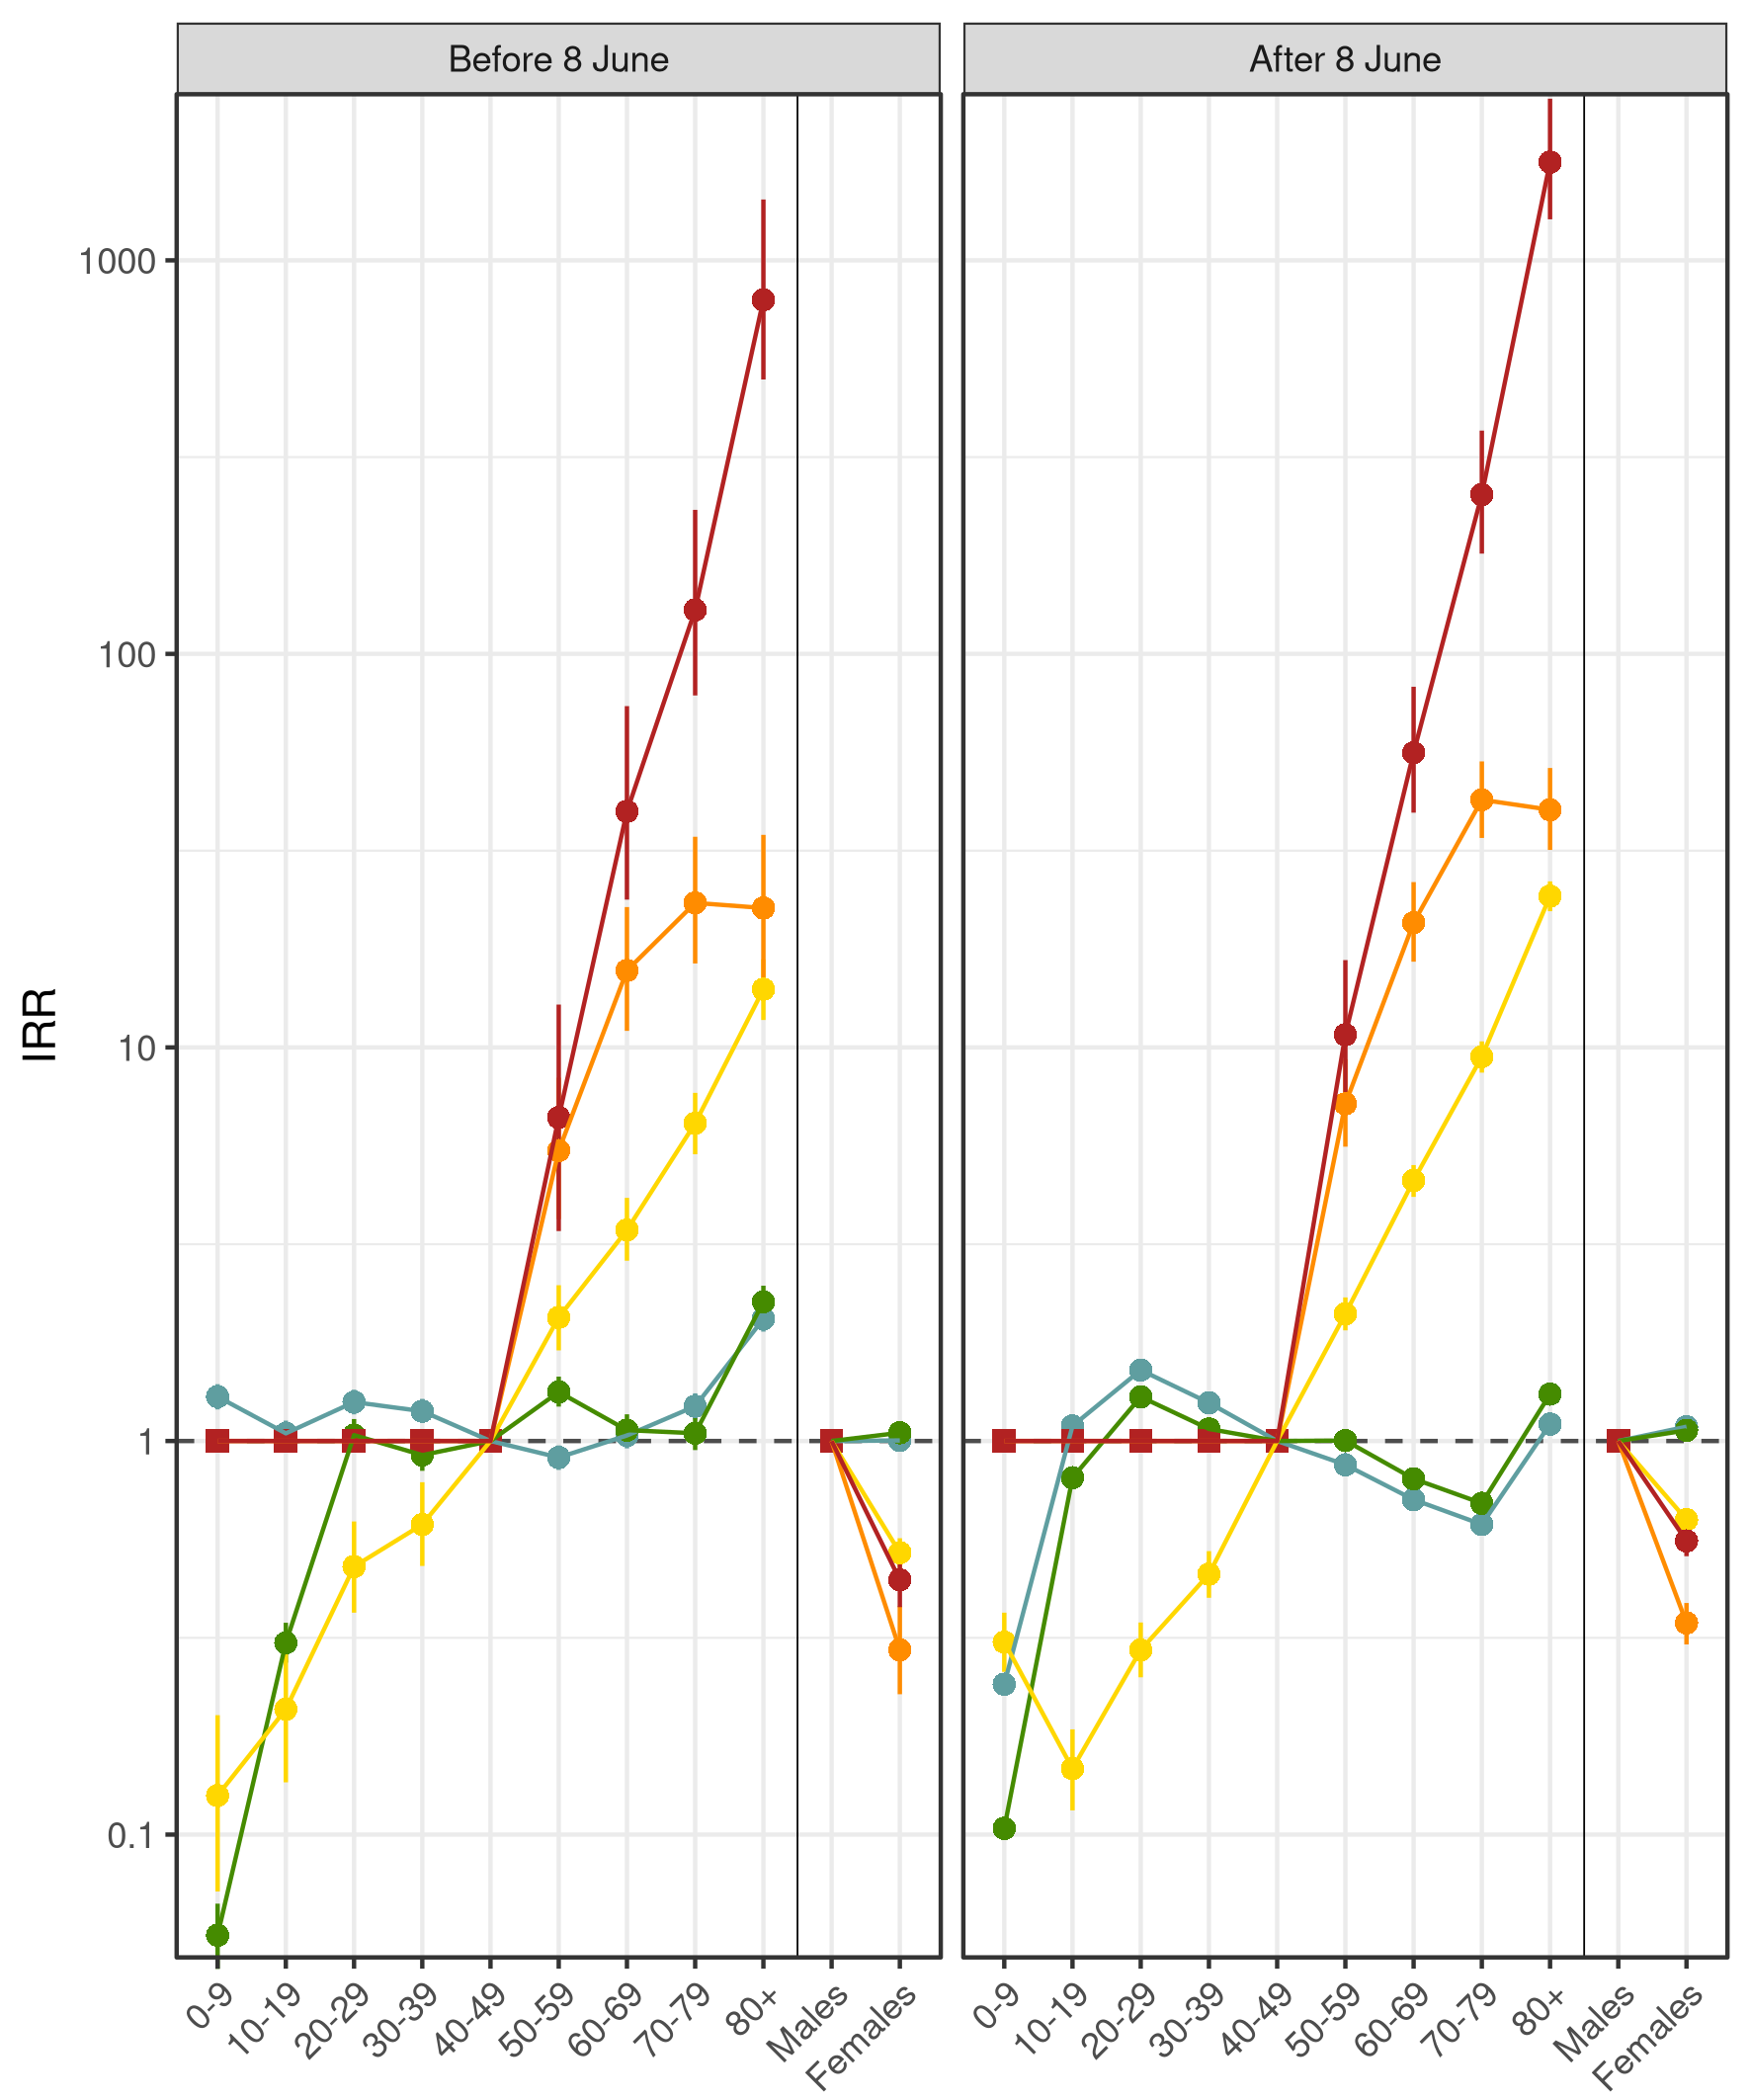
\includegraphics[width=.65\linewidth]{suppfigure_covariates_strat_by_period_8june.png}
		\caption{Estimates of incidence rate ratios between age and sex stratified by epidemic wave.}
		\label{fig:cov_strat}
	\end{figure}
	
	\subsection{Excluding geocodes based only on ZIP code}

	A small proportion of individuals did not provide a full residential address but only a ZIP codes (Table \ref{tab:geocode}). 
	In these situations, the attributed geocode corresponded to the centroïd of the ZIP code area. 
	As ZIP codes might show large heterogeneity with regards to the SEP, this may lead to misclassification and influence the results.
	We repeated the analysis removing these cases from the dataset, and obtained very similar results (Figure \ref{fig:sst}).
	
	
		\begin{figure}[h]
		\centering
		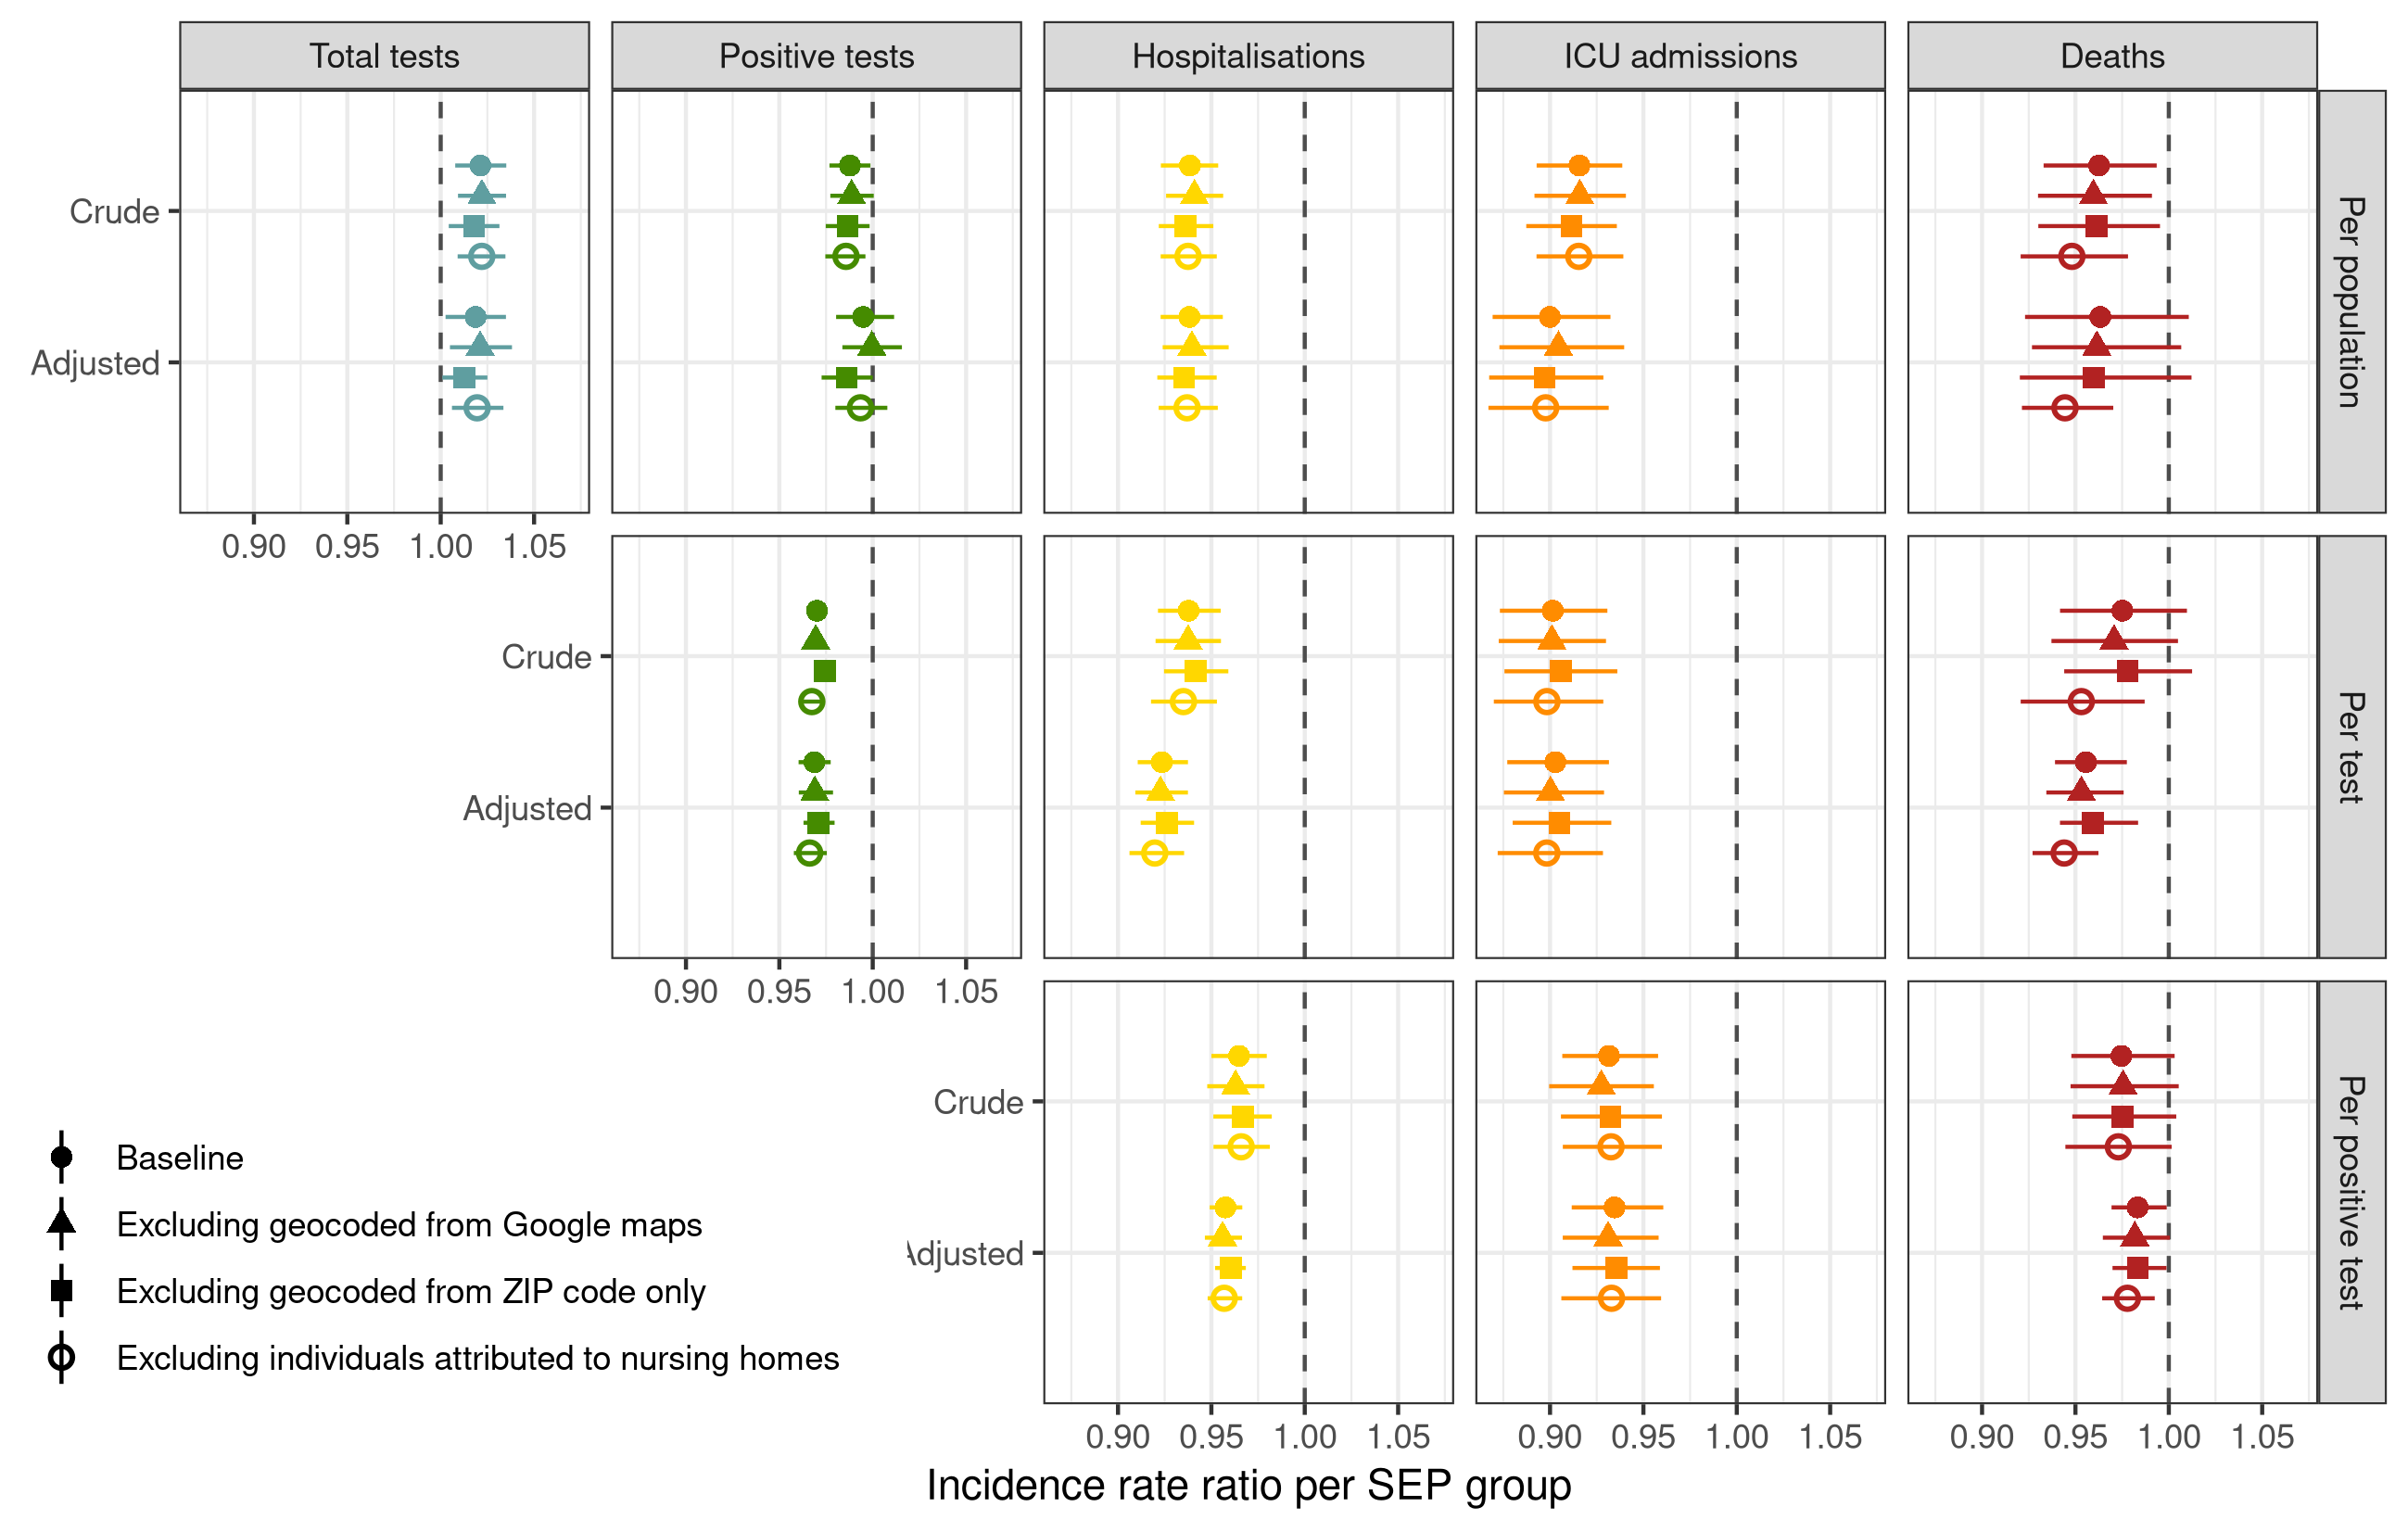
\includegraphics[width=\linewidth]{suppfigure_sensitivity.png}
		\caption{Estimates of incidence rate ratios per decile of SEP in the baseline analysis and in two sensitivity analyses: excluding geocodes based only on ZIP codes only, and excluding geocodes attributed to retirement or nursing homes.}
		\label{fig:sst}
	\end{figure}

	\subsection{Excluding geocodes attributed to retirement or nursing homes}
	
	With our geocoding procedure, residents of retirement or nursing homes are attributed to a SEP decile corresponding to the area of the retirement or nursing home, and not the area where they lived before .
	This may lead to misclassification and influence the results, especially regarding mortality as they may represent a large proportion of deaths.
	Having no direct way of identifying residents of retirements or nursing homes, we considered a sensitivity analysis whereby individuals with addresses geocoded within 25 meters of a retirement or nursing home was excluded (Table \ref{tab:geocode}).
	With this assumption, we identified 1,864 of the COVID-19-related deaths (30.8\%).
	This proportion increased from 11.6\% (129/1,110) during the first wave to 35.1\% (1,735/4,950) during the second wave.
	We also checked the impact of changing the threshold to 50 meters instead of 25 meters. This increased the number of deaths attributed to residents of retirement or nursing homes to 1,993 (32.9\%).
	
	We repeated the analysis removing these cases from the dataset (with the 25 meters threshold).
	The results regarding the association between SEP and tests, positive tests, hospitalisations and ICU admissions were very similar (Figure \ref{fig:sst}).
	Interestingly, removing residents of retirement or nursing homes changed the association between SEP and deaths per population, deaths per test and deaths per positive test.
	In the baseline analysis the association between SEP and mortality was unclear, with a 95\% credible interval including 1 for deaths per population and deaths per positive test.
	Removing these potentially misclassified individuals led to a clear negative association with all three denominators, with 95\% credible intervals excluding 1 in all cases (Table \ref{tab:sst} and \ref{tab:sst2}).
	
	
	\begin{table}[ht]
		\caption{Estimates of incidence rate ratios per decile of SEP in the baseline analysis and in two sensitivity analyses: excluding geocodes based only on ZIP codes only, and excluding geocodes attributed to retirement or nursing homes.}
		\label{tab:sst}
		\centering
		\begin{tabular}{llp{3cm}p{3cm}p{3cm}}
			\hline
			Outcome & Denominator & Baseline & Excluding geocoded from ZIP code only & Excluding individuals attributed to retirement or nursing homes \\ 
			\hline
			Total tests & Per population & 1.02 (1.01-1.04) & 1.01 (1.00-1.03) & 1.02 (1.01-1.04) \\ 
			Positive tests & Per population & 1.00 (0.99-1.02) & 0.99 (0.98-1.01) & 1.00 (0.99-1.02) \\ 
			Positive tests & Per test & 0.97 (0.96-0.98) & 0.97 (0.97-0.98) & 0.97 (0.96-0.98) \\ 
			Hospitalisations & Per population & 0.94 (0.93-0.96) & 0.94 (0.92-0.96) & 0.94 (0.92-0.96) \\ 
			Hospitalisations & Per test & 0.92 (0.91-0.94) & 0.93 (0.91-0.94) & 0.92 (0.91-0.94) \\ 
			Hospitalisations & Per positive test & 0.96 (0.95-0.97) & 0.96 (0.95-0.97) & 0.96 (0.95-0.97) \\ 
			ICU admissions & Per population & 0.90 (0.86-0.94) & 0.90 (0.86-0.93) & 0.90 (0.86-0.94) \\ 
			ICU admissions & Per test & 0.89 (0.87-0.93) & 0.90 (0.87-0.93) & 0.89 (0.86-0.93) \\ 
			ICU admissions & Per positive test & 0.93 (0.90-0.96) & 0.93 (0.90-0.95) & 0.93 (0.90-0.96) \\ 
			Deaths & Per population & 0.97 (0.92-1.02) & 0.96 (0.92-1.01) & 0.95 (0.93-0.99) \\ 
			Deaths & Per test & 0.95 (0.93-0.98) & 0.96 (0.94-0.99) & 0.94 (0.92-0.97) \\ 
			Deaths & Per positive test & 0.98 (0.96-1.00) & 0.98 (0.96-1.00) & 0.98 (0.96-1.00) \\ 
			\hline
		\end{tabular}
	\end{table}
	

\begin{table}[ht]
	\caption{Estimates of incidence rate ratios for the 10th decile of SEP compared to the 1st decile in the baseline analysis and in two sensitivity analyses: excluding geocodes based only on ZIP codes only, and excluding geocodes attributed to retirement or nursing homes.}
	\label{tab:sst2}
	\centering
	\begin{tabular}{llp{3cm}p{3cm}p{3cm}}
		\hline
		Outcome & Denominator & Baseline & Excluding geocoded from ZIP code only & Excluding individuals attributed to retirement or nursing homes \\ 
		\hline
		Total tests & Per population & 1.21 (1.05-1.40) & 1.14 (1.03-1.26) & 1.21 (1.07-1.38) \\ 
		Positive tests & Per population & 1.03 (0.88-1.20) & 0.95 (0.82-1.09) & 1.01 (0.88-1.16) \\ 
		Positive tests & Per test & 0.77 (0.71-0.84) & 0.79 (0.73-0.86) & 0.76 (0.70-0.83) \\ 
		Hospitalisations & Per population & 0.59 (0.50-0.71) & 0.57 (0.49-0.67) & 0.58 (0.49-0.69) \\ 
		Hospitalisations & Per test & 0.49 (0.43-0.57) & 0.51 (0.44-0.60) & 0.48 (0.41-0.55) \\ 
		Hospitalisations & Per positive test & 0.67 (0.61-0.74) & 0.69 (0.63-0.75) & 0.66 (0.61-0.73) \\ 
		ICU admissions & Per population & 0.39 (0.27-0.57) & 0.37 (0.26-0.54) & 0.39 (0.27-0.57) \\ 
		ICU admissions & Per test & 0.37 (0.27-0.50) & 0.38 (0.28-0.53) & 0.36 (0.27-0.50) \\ 
		ICU admissions & Per positive test & 0.50 (0.38-0.66) & 0.50 (0.38-0.65) & 0.50 (0.37-0.67) \\ 
		Deaths & Per population & 0.75 (0.49-1.17) & 0.72 (0.48-1.13) & 0.66 (0.50-0.90) \\ 
		Deaths & Per test & 0.66 (0.54-0.85) & 0.70 (0.55-0.89) & 0.59 (0.48-0.76) \\ 
		Deaths & Per positive test & 0.84 (0.71-1.01) & 0.83 (0.71-1.01) & 0.81 (0.69-0.97) \\
		\hline
	\end{tabular}
\end{table}

	
	\clearpage
	\section{Tables of estimates}
	
	\subsection{Other covariates}
	
	\begin{longtable}{lllc}
		\caption{Incidence rate ratios (95\% credible interval) for the association between age and five outcomes related to SARS-CoV-2 surveillance and care (corresponding to Figure \ref{fig:adj-cov}). The reference group is 40-49 for total tests, positive tests and hospitalisations. Because of the small number of events in younger groups, we pooled together age groups 0 to 49 for ICU admissions and deaths, and used this larger group as reference. The models are also adjusted for sex, epidemic wave, canton and SEP decile.}
		\label{tab:cov-age} \\
		\hline
		Outcome & Denominator & Age group & IRR \\ 
		\hline
		\endfirsthead
			\hline
			Outcome & Denominator & Age group & IRR \\ 
			\hline
			\endhead
			Total tests & population & 0-9 & 0.41 (0.40-0.43) \\ 
			Total tests & population & 10-19 & 1.09 (1.05-1.14) \\ 
			Total tests & population & 0-29 & 1.44 (1.39-1.49) \\ 
			Total tests & population & 30-39 & 1.22 (1.17-1.26) \\ 
			Total tests & population & 50-59 & 0.88 (0.85-0.91) \\ 
			Total tests & population & 60-69 & 0.79 (0.76-0.82) \\ 
			Total tests & population & 70-79 & 0.74 (0.71-0.77) \\ 
			Total tests & population & 80+ & 1.30 (1.25-1.36) \\ 
			Positive tests & population & 0-9 & 0.10 (0.09-0.11) \\ 
			Positive tests & population & 10-19 & 0.69 (0.66-0.72) \\ 
			Positive tests & population & 0-29 & 1.21 (1.16-1.26) \\ 
			Positive tests & population & 30-39 & 1.03 (0.98-1.07) \\ 
			Positive tests & population & 50-59 & 1.10 (1.05-1.15) \\ 
			Positive tests & population & 60-69 & 0.88 (0.84-0.92) \\ 
			Positive tests & population & 70-79 & 0.79 (0.76-0.83) \\ 
			Positive tests & population & 80+ & 1.60 (1.53-1.68) \\ 
			Positive tests & test & 0-9 & 0.43 (0.42-0.45) \\ 
			Positive tests & test & 10-19 & 0.75 (0.73-0.78) \\ 
			Positive tests & test & 0-29 & 0.87 (0.84-0.89) \\ 
			Positive tests & test & 30-39 & 0.87 (0.85-0.89) \\ 
			Positive tests & test & 50-59 & 1.15 (1.12-1.18) \\ 
			Positive tests & test & 60-69 & 1.12 (1.09-1.15) \\ 
			Positive tests & test & 70-79 & 1.11 (1.08-1.15) \\ 
			Positive tests & test & 80+ & 1.21 (1.18-1.24) \\ 
			Hospitalisations & population & 0-9 & 0.27 (0.23-0.31) \\ 
			Hospitalisations & population & 10-19 & 0.16 (0.13-0.20) \\ 
			Hospitalisations & population & 0-29 & 0.33 (0.29-0.38) \\ 
			Hospitalisations & population & 30-39 & 0.49 (0.44-0.55) \\ 
			Hospitalisations & population & 50-59 & 2.11 (1.93-2.31) \\ 
			Hospitalisations & population & 60-69 & 4.30 (3.95-4.68) \\ 
			Hospitalisations & population & 70-79 & 8.68 (8.00-9.44) \\ 
			Hospitalisations & population & 80+ & 21.33 (19.72-23.07) \\ 
			Hospitalisations & test & 0-9 & 1.24 (1.04-1.48) \\ 
			Hospitalisations & test & 10-19 & 0.14 (0.11-0.17) \\ 
			Hospitalisations & test & 0-29 & 0.20 (0.17-0.23) \\ 
			Hospitalisations & test & 30-39 & 0.37 (0.32-0.43) \\ 
			Hospitalisations & test & 50-59 & 2.40 (2.18-2.65) \\ 
			Hospitalisations & test & 60-69 & 6.28 (5.73-6.92) \\ 
			Hospitalisations & test & 70-79 & 14.79 (13.50-16.21) \\ 
			Hospitalisations & test & 80+ & 22.39 (20.50-24.54) \\ 
			Hospitalisations & positive test & 0-9 & 2.63 (2.20-3.12) \\ 
			Hospitalisations & positive test & 10-19 & 0.21 (0.17-0.26) \\ 
			Hospitalisations & positive test & 0-29 & 0.27 (0.23-0.31) \\ 
			Hospitalisations & positive test & 30-39 & 0.47 (0.41-0.52) \\ 
			Hospitalisations & positive test & 50-59 & 2.01 (1.85-2.20) \\ 
			Hospitalisations & positive test & 60-69 & 5.00 (4.58-5.46) \\ 
			Hospitalisations & positive test & 70-79 & 11.30 (10.41-12.28) \\ 
			Hospitalisations & positive test & 80+ & 14.92 (13.78-16.19) \\ 
			ICU admissions & population & 50-59 & 6.86 (5.51-8.56) \\ 
			ICU admissions & population & 60-69 & 19.78 (16.28-24.13) \\ 
			ICU admissions & population & 70-79 & 37.68 (31.22-45.74) \\ 
			ICU admissions & population & 80+ & 35.68 (29.17-44.44) \\ 
			ICU admissions & test & 50-59 & 8.67 (6.74-11.25) \\ 
			ICU admissions & test & 60-69 & 29.35 (23.50-37.05) \\ 
			ICU admissions & test & 70-79 & 66.56 (53.37-83.42) \\ 
			ICU admissions & test & 80+ & 36.61 (29.27-46.46) \\ 
			ICU admissions & positive test & 50-59 & 5.63 (4.55-6.96) \\ 
			ICU admissions & positive test & 60-69 & 18.98 (15.65-22.99) \\ 
			ICU admissions & positive test & 70-79 & 39.68 (33.07-47.95) \\ 
			ICU admissions & positive test & 80+ & 20.29 (16.51-24.82) \\ 
			Deaths & population & 50-59 & 10.35 (7.23-15.28) \\ 
			Deaths & population & 60-69 & 57.05 (42.13-80.47) \\ 
			Deaths & population & 70-79 & 237.52 (176.18-337.08) \\ 
			Deaths & population & 80+ & 1622.59 (1210.26-2280.24) \\ 
			Deaths & test & 50-59 & 12.63 (8.49-19.21) \\ 
			Deaths & test & 60-69 & 79.18 (55.85-115.20) \\ 
			Deaths & test & 70-79 & 403.80 (290.73-578.85) \\ 
			Deaths & test & 80+ & 1636.79 (1180.90-2358.52) \\ 
			Deaths & positive test & 50-59 & 8.88 (6.19-12.75) \\ 
			Deaths & positive test & 60-69 & 58.01 (42.38-80.70) \\ 
			Deaths & positive test & 70-79 & 272.55 (202.08-373.52) \\ 
			Deaths & positive test & 80+ & 944.27 (700.73-1289.76) \\ 
			\hline
		\end{longtable}
	
	
	\begin{table}[H]
		\centering
		\caption{Incidence rate ratios (95\% credible interval) for the association between sex and five outcomes related to SARS-CoV-2 surveillance and care: total tests, positive tests, hospitalisations, intensive care unit (ICU) admissions and deaths. The reference group is males. The models are also adjusted for age, epidemic wave, canton and SEP decile.}
		\label{tab:cov-sex}
		\medskip
		\begin{tabular}{llcc}
			\hline
			Outcome & Denominator & Males & Females \\ 
			\hline
			Total tests & population & - & 1.06 (1.04-1.08) \\ 
			Positive tests & population & - & 1.06 (1.04-1.08) \\ 
			Positive tests & test & - & 0.96 (0.95-0.98) \\ 
			Hospitalisations & population & - & 0.61 (0.58-0.63) \\ 
			Hospitalisations & test & - & 0.58 (0.56-0.61) \\ 
			Hospitalisations & positive test & - & 0.61 (0.59-0.64) \\ 
			ICU admissions & population & - & 0.33 (0.30-0.37) \\ 
			ICU admissions & test & - & 0.33 (0.29-0.37) \\ 
			ICU admissions & positive test & - & 0.35 (0.31-0.39) \\ 
			Deaths & population & - & 0.52 (0.48-0.57) \\ 
			Deaths & test & - & 0.52 (0.47-0.56) \\ 
			Deaths & positive test & - & 0.54 (0.51-0.58) \\ 
			\hline
		\end{tabular}
	\end{table}
	
	\begin{table}[H]
		\centering
		\caption{Incidence rate ratios (95\% credible interval) for the association between epidemic wave and five outcomes related to SARS-CoV-2 surveillance and care: total tests, positive tests, hospitalisations, intensive care unit (ICU) admissions and deaths. The reference group is before 8 June 2020. The models are also adjusted for age, sex, canton and SEP decile.}
		\label{tab:cov-wave}
		\medskip
		\begin{tabular}{llcc}
			\hline
			Outcome & Denominator & Before 8 June 2020 & After 8 June 2020 \\ 
			\hline
			Total tests & population & - & 72.81 (71.31-74.36) \\ 
			Positive tests & population & - & 19.47 (18.98-19.97) \\ 
			Positive tests & test & - & 22.48 (19.86-25.50) \\ 
			Hospitalisations & population & - & 5.12 (4.88-5.37) \\ 
			Hospitalisations & test & - & 9.83 (6.98-14.64) \\ 
			Hospitalisations & positive test & - & 0.38 (0.36-0.40) \\ 
			ICU admissions & population & - & 3.64 (3.23-4.10) \\ 
			ICU admissions & test & - & 7.21 (2.96-22.07) \\ 
			ICU admissions & positive test & - & 0.28 (0.25-0.32) \\ 
			Deaths & population & - & 4.83 (4.38-5.33) \\ 
			Deaths & test & - & 20.34 (9.76-55.83) \\ 
			Deaths & positive test & - & 0.42 (0.39-0.45) \\ 
			\hline
		\end{tabular}
	\end{table}
	
	
	
	\subsection{Interactions}
	
		\begin{longtable}{llll}
			
			\caption{Estimates of interaction between SEP and five outcomes, separately for each covariate (corresponding to figure \ref{fig:slope-cov}). For each combination of outcome, denominator and covariate are shown the interaction term (a value different than 1 indicates an interaction). Estimates correspond to median posterior and 95\% credible interval The reference group for age is 40-49 (squares) for total tests, positive tests and hospitalisations. Because of the small number of events in younger groups, we pooled together age groups 0 to 49 for ICU admissions and deaths, and used this larger group as reference. The reference group is males and the first epidemic wave. }
			\label{tab:slope-cov} \\
			\hline
			Outcome & Denominator & Covariate & Interaction term \\ 
			\hline
			\endfirsthead
			\hline
			Outcome & Denominator & Covariate & Interaction term \\ 
			\hline
			\endhead
		Total tests & population & 0-9 & 0.99 (0.98-1.00) \\ 
		Total tests & population & 10-19 & 0.98 (0.97-1.00) \\ 
		Total tests & population & 0-29 & 0.99 (0.98-1.00) \\ 
		Total tests & population & 30-39 & 1.00 (0.99-1.01) \\ 
		Total tests & population & 50-59 & 0.99 (0.98-1.00) \\ 
		Total tests & population & 60-69 & 0.98 (0.97-1.00) \\ 
		Total tests & population & 70-79 & 0.97 (0.95-0.98) \\ 
		Total tests & population & 80+ & 0.95 (0.94-0.97) \\ 
		Total tests & population & Female & 0.99 (0.99-1.00) \\ 
		Total tests & population & 2nd wave & 1.01 (1.00-1.01) \\ 
		Positive tests & population & 0-9 & 1.04 (1.01-1.06) \\ 
		Positive tests & population & 10-19 & 0.99 (0.98-1.01) \\ 
		Positive tests & population & 0-29 & 1.02 (1.00-1.04) \\ 
		Positive tests & population & 30-39 & 1.02 (1.00-1.03) \\ 
		Positive tests & population & 50-59 & 1.00 (0.98-1.01) \\ 
		Positive tests & population & 60-69 & 0.99 (0.98-1.01) \\ 
		Positive tests & population & 70-79 & 0.97 (0.96-0.99) \\ 
		Positive tests & population & 80+ & 0.97 (0.95-0.98) \\ 
		Positive tests & population & Female & 0.99 (0.98-1.00) \\ 
		Positive tests & population & 2nd wave & 0.96 (0.96-0.97) \\ 
		Positive tests & test & 0-9 & 1.04 (1.02-1.05) \\ 
		Positive tests & test & 10-19 & 1.01 (1.00-1.02) \\ 
		Positive tests & test & 0-29 & 1.02 (1.01-1.03) \\ 
		Positive tests & test & 30-39 & 1.01 (1.00-1.02) \\ 
		Positive tests & test & 50-59 & 1.01 (1.00-1.02) \\ 
		Positive tests & test & 60-69 & 1.01 (1.00-1.02) \\ 
		Positive tests & test & 70-79 & 1.01 (1.00-1.02) \\ 
		Positive tests & test & 80+ & 1.03 (1.02-1.04) \\ 
		Positive tests & test & Female & 1.00 (0.99-1.00) \\ 
		Positive tests & test & 2nd wave & 1.01 (0.96-1.05) \\ 
		Hospitalisations & population & 0-9 & 1.04 (0.98-1.10) \\ 
		Hospitalisations & population & 10-19 & 1.01 (0.93-1.08) \\ 
		Hospitalisations & population & 0-29 & 1.05 (0.99-1.11) \\ 
		Hospitalisations & population & 30-39 & 1.01 (0.96-1.06) \\ 
		Hospitalisations & population & 50-59 & 0.99 (0.96-1.02) \\ 
		Hospitalisations & population & 60-69 & 0.97 (0.94-1.00) \\ 
		Hospitalisations & population & 70-79 & 0.98 (0.95-1.01) \\ 
		Hospitalisations & population & 80+ & 1.02 (0.99-1.05) \\ 
		Hospitalisations & population & Female & 0.99 (0.98-1.01) \\ 
		Hospitalisations & population & 2nd wave & 0.98 (0.96-0.99) \\ 
		Hospitalisations & test & 0-9 & 1.05 (0.99-1.12) \\ 
		Hospitalisations & test & 10-19 & 1.02 (0.94-1.11) \\ 
		Hospitalisations & test & 0-29 & 1.05 (0.99-1.11) \\ 
		Hospitalisations & test & 30-39 & 1.02 (0.97-1.07) \\ 
		Hospitalisations & test & 50-59 & 1.02 (0.98-1.05) \\ 
		Hospitalisations & test & 60-69 & 1.00 (0.96-1.03) \\ 
		Hospitalisations & test & 70-79 & 1.02 (0.99-1.05) \\ 
		Hospitalisations & test & 80+ & 1.09 (1.05-1.12) \\ 
		Hospitalisations & test & Female & 0.99 (0.98-1.01) \\ 
		Hospitalisations & test & 2nd wave & 0.96 (0.84-1.09) \\ 
		Hospitalisations & positive test & 0-9 & 0.99 (0.94-1.05) \\ 
		Hospitalisations & positive test & 10-19 & 1.01 (0.94-1.09) \\ 
		Hospitalisations & positive test & 0-29 & 1.03 (0.98-1.09) \\ 
		Hospitalisations & positive test & 30-39 & 1.00 (0.96-1.04) \\ 
		Hospitalisations & positive test & 50-59 & 0.99 (0.96-1.02) \\ 
		Hospitalisations & positive test & 60-69 & 0.97 (0.95-1.00) \\ 
		Hospitalisations & positive test & 70-79 & 1.00 (0.98-1.03) \\ 
		Hospitalisations & positive test & 80+ & 1.05 (1.02-1.08) \\ 
		Hospitalisations & positive test & Female & 0.99 (0.98-1.01) \\ 
		Hospitalisations & positive test & 2nd wave & 0.99 (0.98-1.01) \\ 
		ICU admissions & population & 50-59 & 1.01 (0.93-1.09) \\ 
		ICU admissions & population & 60-69 & 1.05 (0.98-1.13) \\ 
		ICU admissions & population & 70-79 & 1.03 (0.96-1.10) \\ 
		ICU admissions & population & 80+ & 1.06 (0.98-1.13) \\ 
		ICU admissions & population & Female & 1.00 (0.95-1.04) \\ 
		ICU admissions & population & 2nd wave & 0.98 (0.94-1.03) \\ 
		ICU admissions & test & 50-59 & 0.96 (0.88-1.06) \\ 
		ICU admissions & test & 60-69 & 1.04 (0.96-1.13) \\ 
		ICU admissions & test & 70-79 & 1.05 (0.97-1.13) \\ 
		ICU admissions & test & 80+ & 1.09 (1.00-1.19) \\ 
		ICU admissions & test & Female & 1.01 (0.96-1.06) \\ 
		ICU admissions & test & 2nd wave & 1.04 (0.75-1.50) \\ 
		ICU admissions & positive test & 50-59 & 1.01 (0.93-1.10) \\ 
		ICU admissions & positive test & 60-69 & 1.06 (0.99-1.14) \\ 
		ICU admissions & positive test & 70-79 & 1.07 (1.00-1.15) \\ 
		ICU admissions & positive test & 80+ & 1.09 (1.01-1.17) \\ 
		ICU admissions & positive test & Female & 1.00 (0.96-1.04) \\ 
		ICU admissions & positive test & 2nd wave & 1.01 (0.96-1.05) \\ 
		Deaths & population & 50-59 & 1.04 (0.91-1.19) \\ 
		Deaths & population & 60-69 & 1.05 (0.94-1.19) \\ 
		Deaths & population & 70-79 & 1.03 (0.92-1.16) \\ 
		Deaths & population & 80+ & 1.10 (0.99-1.24) \\ 
		Deaths & population & Female & 1.03 (1.00-1.06) \\ 
		Deaths & population & 2nd wave & 1.00 (0.97-1.03) \\ 
		Deaths & test & 50-59 & 1.02 (0.88-1.20) \\ 
		Deaths & test & 60-69 & 1.04 (0.91-1.21) \\ 
		Deaths & test & 70-79 & 1.02 (0.90-1.18) \\ 
		Deaths & test & 80+ & 1.13 (1.00-1.30) \\ 
		Deaths & test & Female & 1.03 (1.00-1.06) \\ 
		Deaths & test & 2nd wave & 1.19 (0.89-1.72) \\ 
		Deaths & positive test & 50-59 & 1.05 (0.92-1.20) \\ 
		Deaths & positive test & 60-69 & 1.08 (0.96-1.21) \\ 
		Deaths & positive test & 70-79 & 1.07 (0.96-1.20) \\ 
		Deaths & positive test & 80+ & 1.14 (1.02-1.28) \\ 
		Deaths & positive test & Female & 1.02 (1.00-1.04) \\ 
		Deaths & positive test & 2nd wave & 1.01 (0.99-1.04) \\ 
			\hline
		\end{longtable}
	
	\begin{longtable}{lllcc}
		\caption{Estimates of interaction between SEP and five outcomes, separately for each canton (corresponding to figure \ref{fig:slope-canton}). For each combination of outcome, denominator and canton are shown the interaction term (a value different than 1 indicates an interaction) and the incidence rate ratio (computed by multiplying the interaction term by the average effect). Estimates correspond to median posterior and 95\% credible interval.}
		\label{tab:slope-canton} \\
		\hline
		Outcome & Denominator & Canton & Interaction term & IRR \\ 
		\hline
		\endfirsthead
		\hline
		Outcome & Denominator & Canton & Interaction term & IRR \\ 
		\hline
		\endhead
		Total tests & population & AG & 0.99 (0.97-1.01) & 1.01 (0.99-1.02) \\ 
		Positive tests & population & AG & 0.97 (0.94-0.99) & 0.97 (0.95-0.98) \\ 
		Positive tests & test & AG & 0.99 (0.98-1.00) & 0.96 (0.95-0.97) \\ 
		Hospitalisations & population & AG & 0.97 (0.93-1.00) & 0.91 (0.89-0.94) \\ 
		Hospitalisations & test & AG & 0.99 (0.96-1.02) & 0.92 (0.89-0.94) \\ 
		Hospitalisations & positive test & AG & 1.00 (0.97-1.01) & 0.95 (0.93-0.97) \\ 
		ICU admissions & population & AG & 0.98 (0.91-1.05) & 0.88 (0.83-0.95) \\ 
		ICU admissions & test & AG & 1.00 (0.93-1.06) & 0.89 (0.84-0.95) \\ 
		ICU admissions & positive test & AG & 1.00 (0.94-1.06) & 0.92 (0.87-0.98) \\ 
		Deaths & population & AG & 0.96 (0.89-1.04) & 0.93 (0.88-0.99) \\ 
		Deaths & test & AG & 1.01 (0.96-1.06) & 0.96 (0.92-1.01) \\ 
		Deaths & positive test & AG & 1.01 (0.97-1.05) & 0.99 (0.95-1.03) \\ 
		Total tests & population & AI & 1.05 (1.01-1.08) & 1.07 (1.04-1.10) \\ 
		Positive tests & population & AI & 1.08 (1.03-1.13) & 1.08 (1.04-1.13) \\ 
		Positive tests & test & AI & 1.03 (1.00-1.06) & 1.00 (0.97-1.03) \\ 
		Hospitalisations & population & AI & 1.02 (0.96-1.11) & 0.96 (0.90-1.05) \\ 
		Hospitalisations & test & AI & 1.01 (0.95-1.07) & 0.93 (0.88-0.99) \\ 
		Hospitalisations & positive test & AI & 1.00 (0.97-1.03) & 0.96 (0.93-0.99) \\ 
		ICU admissions & population & AI & 0.99 (0.86-1.15) & 0.89 (0.77-1.04) \\ 
		ICU admissions & test & AI & 1.00 (0.90-1.11) & 0.89 (0.80-1.00) \\ 
		ICU admissions & positive test & AI & 1.00 (0.91-1.11) & 0.93 (0.84-1.03) \\ 
		Deaths & population & AI & 1.04 (0.88-1.25) & 1.01 (0.85-1.22) \\ 
		Deaths & test & AI & 1.00 (0.92-1.08) & 0.95 (0.88-1.04) \\ 
		Deaths & positive test & AI & 1.02 (0.96-1.10) & 1.00 (0.94-1.08) \\ 
		Total tests & population & AR & 0.99 (0.97-1.02) & 1.01 (0.99-1.03) \\ 
		Positive tests & population & AR & 1.00 (0.97-1.03) & 1.01 (0.98-1.03) \\ 
		Positive tests & test & AR & 1.01 (0.99-1.03) & 0.99 (0.97-1.00) \\ 
		Hospitalisations & population & AR & 1.02 (0.97-1.09) & 0.97 (0.92-1.02) \\ 
		Hospitalisations & test & AR & 1.02 (0.98-1.08) & 0.94 (0.90-1.00) \\ 
		Hospitalisations & positive test & AR & 1.00 (0.97-1.04) & 0.96 (0.93-0.99) \\ 
		ICU admissions & population & AR & 1.04 (0.94-1.16) & 0.94 (0.84-1.05) \\ 
		ICU admissions & test & AR & 1.02 (0.93-1.15) & 0.91 (0.83-1.04) \\ 
		ICU admissions & positive test & AR & 1.00 (0.92-1.10) & 0.93 (0.85-1.02) \\ 
		Deaths & population & AR & 0.97 (0.85-1.09) & 0.94 (0.84-1.05) \\ 
		Deaths & test & AR & 1.00 (0.92-1.08) & 0.95 (0.88-1.03) \\ 
		Deaths & positive test & AR & 0.99 (0.93-1.04) & 0.97 (0.91-1.02) \\ 
		Total tests & population & BE & 1.05 (1.03-1.07) & 1.08 (1.06-1.09) \\ 
		Positive tests & population & BE & 1.01 (0.99-1.03) & 1.01 (1.00-1.03) \\ 
		Positive tests & test & BE & 0.98 (0.96-0.99) & 0.95 (0.94-0.96) \\ 
		Hospitalisations & population & BE & 0.99 (0.96-1.02) & 0.93 (0.91-0.96) \\ 
		Hospitalisations & test & BE & 0.97 (0.94-1.00) & 0.90 (0.88-0.92) \\ 
		Hospitalisations & positive test & BE & 0.99 (0.97-1.01) & 0.95 (0.93-0.96) \\ 
		ICU admissions & population & BE & 0.99 (0.93-1.06) & 0.89 (0.84-0.94) \\ 
		ICU admissions & test & BE & 0.98 (0.92-1.03) & 0.88 (0.83-0.92) \\ 
		ICU admissions & positive test & BE & 0.98 (0.93-1.03) & 0.91 (0.86-0.95) \\ 
		Deaths & population & BE & 1.01 (0.95-1.08) & 0.98 (0.93-1.03) \\ 
		Deaths & test & BE & 1.02 (0.97-1.07) & 0.97 (0.93-1.02) \\ 
		Deaths & positive test & BE & 1.01 (0.98-1.05) & 0.99 (0.96-1.03) \\ 
		Total tests & population & BL & 0.96 (0.94-0.98) & 0.98 (0.97-0.99) \\ 
		Positive tests & population & BL & 0.95 (0.93-0.98) & 0.96 (0.94-0.97) \\ 
		Positive tests & test & BL & 0.99 (0.97-1.00) & 0.96 (0.95-0.97) \\ 
		Hospitalisations & population & BL & 0.96 (0.93-1.00) & 0.91 (0.88-0.94) \\ 
		Hospitalisations & test & BL & 1.01 (0.98-1.05) & 0.94 (0.91-0.97) \\ 
		Hospitalisations & positive test & BL & 1.00 (0.98-1.03) & 0.96 (0.94-0.99) \\ 
		ICU admissions & population & BL & 0.94 (0.86-1.01) & 0.85 (0.78-0.91) \\ 
		ICU admissions & test & BL & 0.98 (0.89-1.05) & 0.88 (0.80-0.94) \\ 
		ICU admissions & positive test & BL & 0.98 (0.90-1.05) & 0.91 (0.84-0.97) \\ 
		Deaths & population & BL & 0.87 (0.80-0.94) & 0.84 (0.78-0.90) \\ 
		Deaths & test & BL & 0.97 (0.91-1.03) & 0.93 (0.87-0.98) \\ 
		Deaths & positive test & BL & 0.98 (0.93-1.03) & 0.97 (0.92-1.01) \\ 
		Total tests & population & BS & 0.99 (0.97-1.01) & 1.01 (0.99-1.02) \\ 
		Positive tests & population & BS & 1.01 (0.98-1.03) & 1.01 (0.99-1.03) \\ 
		Positive tests & test & BS & 0.97 (0.95-0.98) & 0.94 (0.93-0.95) \\ 
		Hospitalisations & population & BS & 0.97 (0.94-1.01) & 0.92 (0.89-0.94) \\ 
		Hospitalisations & test & BS & 0.97 (0.94-1.01) & 0.90 (0.87-0.93) \\ 
		Hospitalisations & positive test & BS & 0.99 (0.97-1.01) & 0.95 (0.93-0.97) \\ 
		ICU admissions & population & BS & 0.95 (0.86-1.04) & 0.86 (0.78-0.93) \\ 
		ICU admissions & test & BS & 0.97 (0.87-1.04) & 0.87 (0.78-0.93) \\ 
		ICU admissions & positive test & BS & 0.96 (0.88-1.02) & 0.89 (0.81-0.95) \\ 
		Deaths & population & BS & 0.94 (0.86-1.02) & 0.91 (0.84-0.97) \\ 
		Deaths & test & BS & 0.96 (0.88-1.01) & 0.92 (0.85-0.97) \\ 
		Deaths & positive test & BS & 0.97 (0.92-1.01) & 0.95 (0.91-0.99) \\ 
		Total tests & population & FR & 0.98 (0.96-1.01) & 1.01 (0.99-1.02) \\ 
		Positive tests & population & FR & 0.98 (0.96-1.00) & 0.98 (0.97-1.00) \\ 
		Positive tests & test & FR & 1.01 (1.00-1.03) & 0.98 (0.97-0.99) \\ 
		Hospitalisations & population & FR & 1.02 (0.99-1.06) & 0.96 (0.93-1.00) \\ 
		Hospitalisations & test & FR & 1.03 (1.00-1.07) & 0.95 (0.92-0.99) \\ 
		Hospitalisations & positive test & FR & 1.01 (0.99-1.05) & 0.97 (0.95-1.00) \\ 
		ICU admissions & population & FR & 1.12 (1.04-1.21) & 1.01 (0.94-1.08) \\ 
		ICU admissions & test & FR & 1.06 (0.99-1.17) & 0.95 (0.88-1.04) \\ 
		ICU admissions & positive test & FR & 1.07 (0.99-1.17) & 0.99 (0.92-1.08) \\ 
		Deaths & population & FR & 0.93 (0.85-1.00) & 0.90 (0.83-0.96) \\ 
		Deaths & test & FR & 0.98 (0.92-1.03) & 0.93 (0.88-0.98) \\ 
		Deaths & positive test & FR & 0.99 (0.94-1.02) & 0.97 (0.92-1.00) \\ 
		Total tests & population & GE & 1.10 (1.08-1.12) & 1.12 (1.11-1.14) \\ 
		Positive tests & population & GE & 1.08 (1.06-1.11) & 1.09 (1.07-1.10) \\ 
		Positive tests & test & GE & 0.97 (0.95-0.98) & 0.94 (0.93-0.95) \\ 
		Hospitalisations & population & GE & 1.07 (1.03-1.10) & 1.01 (0.98-1.04) \\ 
		Hospitalisations & test & GE & 1.00 (0.96-1.03) & 0.92 (0.89-0.95) \\ 
		Hospitalisations & positive test & GE & 1.01 (0.99-1.03) & 0.97 (0.95-0.99) \\ 
		ICU admissions & population & GE & 1.11 (1.04-1.18) & 1.00 (0.94-1.05) \\ 
		ICU admissions & test & GE & 1.01 (0.95-1.07) & 0.90 (0.86-0.96) \\ 
		ICU admissions & positive test & GE & 1.02 (0.97-1.08) & 0.95 (0.90-0.99) \\ 
		Deaths & population & GE & 1.09 (1.01-1.16) & 1.05 (1.00-1.11) \\ 
		Deaths & test & GE & 0.99 (0.95-1.04) & 0.95 (0.91-0.99) \\ 
		Deaths & positive test & GE & 1.01 (0.98-1.05) & 0.99 (0.96-1.02) \\ 
		Total tests & population & GL & 1.01 (0.98-1.04) & 1.03 (1.01-1.06) \\ 
		Positive tests & population & GL & 1.03 (0.99-1.07) & 1.03 (1.00-1.07) \\ 
		Positive tests & test & GL & 1.01 (0.98-1.03) & 0.98 (0.95-1.00) \\ 
		Hospitalisations & population & GL & 1.00 (0.94-1.07) & 0.94 (0.88-1.01) \\ 
		Hospitalisations & test & GL & 0.99 (0.94-1.04) & 0.92 (0.87-0.96) \\ 
		Hospitalisations & positive test & GL & 0.99 (0.95-1.02) & 0.95 (0.91-0.98) \\ 
		ICU admissions & population & GL & 1.06 (0.94-1.21) & 0.95 (0.84-1.09) \\ 
		ICU admissions & test & GL & 1.01 (0.93-1.14) & 0.91 (0.83-1.02) \\ 
		ICU admissions & positive test & GL & 0.99 (0.89-1.10) & 0.92 (0.83-1.02) \\ 
		Deaths & population & GL & 1.05 (0.91-1.21) & 1.02 (0.89-1.16) \\ 
		Deaths & test & GL & 1.00 (0.92-1.09) & 0.96 (0.88-1.04) \\ 
		Deaths & positive test & GL & 0.98 (0.91-1.04) & 0.96 (0.90-1.02) \\ 
		Total tests & population & GR & 1.02 (0.99-1.04) & 1.04 (1.02-1.05) \\ 
		Positive tests & population & GR & 0.99 (0.96-1.02) & 0.99 (0.97-1.01) \\ 
		Positive tests & test & GR & 1.00 (0.99-1.02) & 0.98 (0.96-0.99) \\ 
		Hospitalisations & population & GR & 1.01 (0.97-1.06) & 0.96 (0.92-1.00) \\ 
		Hospitalisations & test & GR & 1.00 (0.95-1.03) & 0.92 (0.88-0.96) \\ 
		Hospitalisations & positive test & GR & 1.00 (0.98-1.03) & 0.96 (0.94-0.99) \\ 
		ICU admissions & population & GR & 0.97 (0.87-1.07) & 0.87 (0.79-0.96) \\ 
		ICU admissions & test & GR & 0.99 (0.90-1.09) & 0.89 (0.80-0.98) \\ 
		ICU admissions & positive test & GR & 0.99 (0.91-1.06) & 0.92 (0.84-0.98) \\ 
		Deaths & population & GR & 1.00 (0.91-1.09) & 0.96 (0.88-1.05) \\ 
		Deaths & test & GR & 1.01 (0.95-1.08) & 0.96 (0.90-1.04) \\ 
		Deaths & positive test & GR & 1.02 (0.98-1.08) & 1.00 (0.96-1.06) \\ 
		Total tests & population & JU & 0.98 (0.95-1.00) & 1.00 (0.98-1.02) \\ 
		Positive tests & population & JU & 1.03 (1.00-1.07) & 1.04 (1.01-1.07) \\ 
		Positive tests & test & JU & 1.02 (1.00-1.04) & 0.99 (0.97-1.01) \\ 
		Hospitalisations & population & JU & 1.02 (0.96-1.08) & 0.96 (0.90-1.02) \\ 
		Hospitalisations & test & JU & 0.99 (0.93-1.04) & 0.91 (0.86-0.96) \\ 
		Hospitalisations & positive test & JU & 1.00 (0.97-1.03) & 0.96 (0.92-0.99) \\ 
		ICU admissions & population & JU & 1.02 (0.91-1.17) & 0.92 (0.81-1.05) \\ 
		ICU admissions & test & JU & 1.00 (0.90-1.10) & 0.89 (0.81-0.99) \\ 
		ICU admissions & positive test & JU & 1.00 (0.92-1.10) & 0.93 (0.85-1.02) \\ 
		Deaths & population & JU & 1.03 (0.89-1.19) & 1.00 (0.86-1.15) \\ 
		Deaths & test & JU & 1.00 (0.91-1.09) & 0.95 (0.87-1.05) \\ 
		Deaths & positive test & JU & 1.04 (0.97-1.11) & 1.02 (0.95-1.09) \\ 
		Total tests & population & LU & 1.01 (0.99-1.03) & 1.03 (1.02-1.04) \\ 
		Positive tests & population & LU & 0.98 (0.96-1.00) & 0.99 (0.97-1.00) \\ 
		Positive tests & test & LU & 0.98 (0.96-0.99) & 0.95 (0.94-0.96) \\ 
		Hospitalisations & population & LU & 0.98 (0.94-1.02) & 0.92 (0.89-0.95) \\ 
		Hospitalisations & test & LU & 0.99 (0.95-1.02) & 0.91 (0.88-0.94) \\ 
		Hospitalisations & positive test & LU & 1.00 (0.98-1.02) & 0.96 (0.94-0.98) \\ 
		ICU admissions & population & LU & 0.99 (0.92-1.07) & 0.89 (0.83-0.96) \\ 
		ICU admissions & test & LU & 1.00 (0.93-1.06) & 0.89 (0.83-0.95) \\ 
		ICU admissions & positive test & LU & 1.00 (0.93-1.07) & 0.93 (0.86-0.99) \\ 
		Deaths & population & LU & 0.95 (0.88-1.02) & 0.92 (0.86-0.98) \\ 
		Deaths & test & LU & 0.98 (0.92-1.02) & 0.93 (0.88-0.98) \\ 
		Deaths & positive test & LU & 1.00 (0.96-1.03) & 0.98 (0.94-1.01) \\ 
		Total tests & population & NE & 0.97 (0.94-0.99) & 0.99 (0.97-1.00) \\ 
		Positive tests & population & NE & 0.99 (0.96-1.01) & 0.99 (0.97-1.01) \\ 
		Positive tests & test & NE & 1.02 (1.00-1.03) & 0.99 (0.98-1.00) \\ 
		Hospitalisations & population & NE & 0.97 (0.92-1.01) & 0.91 (0.87-0.96) \\ 
		Hospitalisations & test & NE & 0.99 (0.94-1.04) & 0.92 (0.87-0.96) \\ 
		Hospitalisations & positive test & NE & 1.00 (0.96-1.03) & 0.96 (0.92-0.98) \\ 
		ICU admissions & population & NE & 1.01 (0.91-1.11) & 0.91 (0.83-1.00) \\ 
		ICU admissions & test & NE & 1.00 (0.91-1.08) & 0.89 (0.81-0.97) \\ 
		ICU admissions & positive test & NE & 1.01 (0.93-1.09) & 0.93 (0.87-1.01) \\ 
		Deaths & population & NE & 0.94 (0.86-1.03) & 0.91 (0.84-0.99) \\ 
		Deaths & test & NE & 0.98 (0.92-1.04) & 0.94 (0.88-0.99) \\ 
		Deaths & positive test & NE & 1.00 (0.95-1.04) & 0.98 (0.93-1.02) \\ 
		Total tests & population & NW & 1.00 (0.98-1.03) & 1.02 (1.00-1.04) \\ 
		Positive tests & population & NW & 0.99 (0.96-1.02) & 0.99 (0.96-1.02) \\ 
		Positive tests & test & NW & 1.00 (0.98-1.03) & 0.98 (0.96-1.00) \\ 
		Hospitalisations & population & NW & 1.02 (0.97-1.09) & 0.96 (0.91-1.03) \\ 
		Hospitalisations & test & NW & 1.01 (0.96-1.06) & 0.93 (0.89-0.98) \\ 
		Hospitalisations & positive test & NW & 1.00 (0.98-1.04) & 0.96 (0.93-0.99) \\ 
		ICU admissions & population & NW & 0.96 (0.83-1.09) & 0.86 (0.75-0.98) \\ 
		ICU admissions & test & NW & 1.00 (0.90-1.10) & 0.89 (0.80-0.99) \\ 
		ICU admissions & positive test & NW & 1.00 (0.91-1.12) & 0.93 (0.84-1.04) \\ 
		Deaths & population & NW & 1.03 (0.89-1.22) & 1.00 (0.86-1.18) \\ 
		Deaths & test & NW & 1.01 (0.94-1.11) & 0.96 (0.89-1.06) \\ 
		Deaths & positive test & NW & 1.02 (0.96-1.10) & 1.00 (0.94-1.08) \\ 
		Total tests & population & OW & 1.04 (1.02-1.07) & 1.07 (1.04-1.09) \\ 
		Positive tests & population & OW & 1.03 (0.99-1.07) & 1.03 (1.00-1.07) \\ 
		Positive tests & test & OW & 0.99 (0.97-1.02) & 0.96 (0.94-0.99) \\ 
		Hospitalisations & population & OW & 1.02 (0.96-1.10) & 0.97 (0.91-1.04) \\ 
		Hospitalisations & test & OW & 0.99 (0.94-1.04) & 0.92 (0.87-0.96) \\ 
		Hospitalisations & positive test & OW & 1.00 (0.96-1.02) & 0.95 (0.92-0.98) \\ 
		ICU admissions & population & OW & 1.00 (0.88-1.15) & 0.90 (0.79-1.05) \\ 
		ICU admissions & test & OW & 1.01 (0.92-1.13) & 0.90 (0.82-1.01) \\ 
		ICU admissions & positive test & OW & 1.01 (0.92-1.13) & 0.94 (0.85-1.05) \\ 
		Deaths & population & OW & 1.26 (1.07-1.51) & 1.22 (1.04-1.47) \\ 
		Deaths & test & OW & 1.03 (0.96-1.14) & 0.98 (0.92-1.10) \\ 
		Deaths & positive test & OW & 1.02 (0.97-1.09) & 1.00 (0.94-1.07) \\ 
		Total tests & population & SG & 0.97 (0.95-0.99) & 1.00 (0.98-1.01) \\ 
		Positive tests & population & SG & 1.02 (1.00-1.04) & 1.02 (1.01-1.04) \\ 
		Positive tests & test & SG & 1.03 (1.02-1.04) & 1.00 (0.99-1.01) \\ 
		Hospitalisations & population & SG & 1.02 (0.99-1.05) & 0.96 (0.94-0.99) \\ 
		Hospitalisations & test & SG & 1.02 (1.00-1.06) & 0.95 (0.92-0.97) \\ 
		Hospitalisations & positive test & SG & 1.01 (0.99-1.03) & 0.96 (0.95-0.99) \\ 
		ICU admissions & population & SG & 1.02 (0.95-1.10) & 0.92 (0.86-0.99) \\ 
		ICU admissions & test & SG & 1.01 (0.95-1.09) & 0.91 (0.85-0.97) \\ 
		ICU admissions & positive test & SG & 1.01 (0.95-1.08) & 0.94 (0.88-1.00) \\ 
		Deaths & population & SG & 0.99 (0.92-1.06) & 0.96 (0.91-1.01) \\ 
		Deaths & test & SG & 1.01 (0.96-1.06) & 0.96 (0.92-1.01) \\ 
		Deaths & positive test & SG & 0.99 (0.95-1.02) & 0.97 (0.94-1.00) \\ 
		Total tests & population & SH & 0.98 (0.96-1.01) & 1.00 (0.99-1.02) \\ 
		Positive tests & population & SH & 0.96 (0.94-0.99) & 0.97 (0.94-0.99) \\ 
		Positive tests & test & SH & 0.98 (0.96-1.00) & 0.95 (0.94-0.97) \\ 
		Hospitalisations & population & SH & 1.00 (0.94-1.05) & 0.94 (0.89-0.99) \\ 
		Hospitalisations & test & SH & 1.01 (0.97-1.05) & 0.93 (0.89-0.97) \\ 
		Hospitalisations & positive test & SH & 1.00 (0.98-1.04) & 0.96 (0.93-0.99) \\ 
		ICU admissions & population & SH & 0.94 (0.82-1.06) & 0.85 (0.74-0.96) \\ 
		ICU admissions & test & SH & 0.99 (0.89-1.08) & 0.89 (0.80-0.98) \\ 
		ICU admissions & positive test & SH & 1.00 (0.90-1.10) & 0.92 (0.83-1.02) \\ 
		Deaths & population & SH & 1.03 (0.92-1.15) & 1.00 (0.89-1.11) \\ 
		Deaths & test & SH & 1.02 (0.96-1.11) & 0.97 (0.92-1.06) \\ 
		Deaths & positive test & SH & 1.01 (0.95-1.07) & 0.99 (0.93-1.05) \\ 
		Total tests & population & SO & 0.99 (0.97-1.01) & 1.01 (1.00-1.03) \\ 
		Positive tests & population & SO & 0.97 (0.95-1.00) & 0.98 (0.96-1.00) \\ 
		Positive tests & test & SO & 0.98 (0.96-0.99) & 0.95 (0.94-0.96) \\ 
		Hospitalisations & population & SO & 0.96 (0.92-0.99) & 0.90 (0.88-0.94) \\ 
		Hospitalisations & test & SO & 0.98 (0.94-1.01) & 0.90 (0.87-0.93) \\ 
		Hospitalisations & positive test & SO & 0.99 (0.96-1.01) & 0.95 (0.92-0.97) \\ 
		ICU admissions & population & SO & 0.96 (0.88-1.04) & 0.87 (0.79-0.93) \\ 
		ICU admissions & test & SO & 0.99 (0.90-1.06) & 0.88 (0.80-0.95) \\ 
		ICU admissions & positive test & SO & 0.97 (0.90-1.04) & 0.90 (0.83-0.96) \\ 
		Deaths & population & SO & 0.97 (0.89-1.05) & 0.94 (0.87-1.01) \\ 
		Deaths & test & SO & 1.01 (0.95-1.06) & 0.96 (0.91-1.02) \\ 
		Deaths & positive test & SO & 1.01 (0.97-1.05) & 0.99 (0.95-1.04) \\ 
		Total tests & population & SZ & 1.00 (0.98-1.02) & 1.02 (1.01-1.04) \\ 
		Positive tests & population & SZ & 0.98 (0.96-1.01) & 0.98 (0.97-1.00) \\ 
		Positive tests & test & SZ & 0.99 (0.97-1.00) & 0.96 (0.95-0.97) \\ 
		Hospitalisations & population & SZ & 0.99 (0.95-1.03) & 0.94 (0.90-0.97) \\ 
		Hospitalisations & test & SZ & 0.99 (0.96-1.03) & 0.92 (0.89-0.95) \\ 
		Hospitalisations & positive test & SZ & 1.00 (0.98-1.03) & 0.96 (0.93-0.98) \\ 
		ICU admissions & population & SZ & 0.99 (0.90-1.08) & 0.89 (0.81-0.97) \\ 
		ICU admissions & test & SZ & 0.98 (0.89-1.05) & 0.88 (0.80-0.94) \\ 
		ICU admissions & positive test & SZ & 0.98 (0.91-1.05) & 0.91 (0.84-0.97) \\ 
		Deaths & population & SZ & 0.96 (0.88-1.05) & 0.93 (0.86-1.00) \\ 
		Deaths & test & SZ & 0.99 (0.92-1.04) & 0.94 (0.88-0.99) \\ 
		Deaths & positive test & SZ & 0.98 (0.93-1.02) & 0.96 (0.92-1.01) \\ 
		Total tests & population & TG & 0.97 (0.95-0.99) & 0.99 (0.98-1.01) \\ 
		Positive tests & population & TG & 0.97 (0.95-1.00) & 0.98 (0.96-0.99) \\ 
		Positive tests & test & TG & 1.01 (0.99-1.02) & 0.98 (0.97-0.99) \\ 
		Hospitalisations & population & TG & 0.96 (0.92-1.00) & 0.91 (0.87-0.94) \\ 
		Hospitalisations & test & TG & 1.00 (0.96-1.04) & 0.93 (0.89-0.96) \\ 
		Hospitalisations & positive test & TG & 0.99 (0.96-1.01) & 0.95 (0.92-0.97) \\ 
		ICU admissions & population & TG & 0.98 (0.89-1.06) & 0.88 (0.80-0.95) \\ 
		ICU admissions & test & TG & 1.00 (0.93-1.08) & 0.90 (0.83-0.97) \\ 
		ICU admissions & positive test & TG & 0.97 (0.90-1.05) & 0.90 (0.83-0.96) \\ 
		Deaths & population & TG & 0.89 (0.81-0.96) & 0.86 (0.80-0.92) \\ 
		Deaths & test & TG & 0.98 (0.92-1.04) & 0.94 (0.88-0.99) \\ 
		Deaths & positive test & TG & 0.96 (0.90-1.00) & 0.94 (0.89-0.98) \\ 
		Total tests & population & TI & 0.99 (0.97-1.01) & 1.01 (0.99-1.02) \\ 
		Positive tests & population & TI & 0.95 (0.93-0.98) & 0.95 (0.94-0.97) \\ 
		Positive tests & test & TI & 1.01 (1.00-1.03) & 0.98 (0.97-0.99) \\ 
		Hospitalisations & population & TI & 0.98 (0.95-1.01) & 0.92 (0.90-0.95) \\ 
		Hospitalisations & test & TI & 1.02 (0.99-1.05) & 0.94 (0.92-0.97) \\ 
		Hospitalisations & positive test & TI & 1.00 (0.98-1.02) & 0.96 (0.94-0.98) \\ 
		ICU admissions & population & TI & 1.00 (0.92-1.09) & 0.91 (0.84-0.97) \\ 
		ICU admissions & test & TI & 1.01 (0.95-1.10) & 0.90 (0.85-0.98) \\ 
		ICU admissions & positive test & TI & 1.00 (0.94-1.06) & 0.93 (0.87-0.99) \\ 
		Deaths & population & TI & 0.92 (0.85-0.99) & 0.89 (0.83-0.95) \\ 
		Deaths & test & TI & 1.01 (0.96-1.07) & 0.96 (0.92-1.02) \\ 
		Deaths & positive test & TI & 0.99 (0.95-1.02) & 0.97 (0.94-1.00) \\ 
		Total tests & population & UR & 1.07 (1.04-1.10) & 1.09 (1.07-1.12) \\ 
		Positive tests & population & UR & 1.09 (1.06-1.14) & 1.10 (1.06-1.13) \\ 
		Positive tests & test & UR & 1.03 (1.01-1.06) & 1.00 (0.98-1.02) \\ 
		Hospitalisations & population & UR & 1.05 (0.99-1.14) & 0.99 (0.93-1.08) \\ 
		Hospitalisations & test & UR & 1.01 (0.96-1.06) & 0.93 (0.88-0.98) \\ 
		Hospitalisations & positive test & UR & 1.00 (0.97-1.03) & 0.96 (0.93-0.99) \\ 
		ICU admissions & population & UR & 0.99 (0.85-1.14) & 0.89 (0.77-1.04) \\ 
		ICU admissions & test & UR & 1.00 (0.90-1.11) & 0.89 (0.81-1.00) \\ 
		ICU admissions & positive test & UR & 1.01 (0.92-1.12) & 0.93 (0.84-1.04) \\ 
		Deaths & population & UR & 1.24 (1.08-1.45) & 1.20 (1.04-1.41) \\ 
		Deaths & test & UR & 1.03 (0.97-1.15) & 0.98 (0.92-1.10) \\ 
		Deaths & positive test & UR & 1.01 (0.96-1.07) & 0.99 (0.94-1.06) \\ 
		Total tests & population & VD & 0.97 (0.95-0.99) & 0.99 (0.98-1.00) \\ 
		Positive tests & population & VD & 1.00 (0.98-1.03) & 1.00 (0.99-1.02) \\ 
		Positive tests & test & VD & 1.02 (1.00-1.03) & 0.99 (0.98-1.00) \\ 
		Hospitalisations & population & VD & 1.01 (0.98-1.04) & 0.95 (0.93-0.97) \\ 
		Hospitalisations & test & VD & 1.01 (0.99-1.04) & 0.94 (0.92-0.96) \\ 
		Hospitalisations & positive test & VD & 1.00 (0.99-1.02) & 0.96 (0.95-0.98) \\ 
		ICU admissions & population & VD & 1.01 (0.95-1.08) & 0.91 (0.86-0.96) \\ 
		ICU admissions & test & VD & 1.00 (0.94-1.07) & 0.90 (0.85-0.95) \\ 
		ICU admissions & positive test & VD & 1.00 (0.95-1.06) & 0.93 (0.88-0.97) \\ 
		Deaths & population & VD & 1.00 (0.93-1.07) & 0.97 (0.92-1.02) \\ 
		Deaths & test & VD & 1.00 (0.96-1.05) & 0.96 (0.92-1.00) \\ 
		Deaths & positive test & VD & 1.01 (0.98-1.04) & 0.99 (0.96-1.02) \\ 
		Total tests & population & VS & 0.97 (0.94-0.99) & 0.99 (0.97-1.01) \\ 
		Positive tests & population & VS & 0.99 (0.96-1.02) & 0.99 (0.97-1.01) \\ 
		Positive tests & test & VS & 1.03 (1.02-1.05) & 1.00 (0.99-1.02) \\ 
		Hospitalisations & population & VS & 1.04 (1.00-1.09) & 0.99 (0.95-1.03) \\ 
		Hospitalisations & test & VS & 1.04 (1.00-1.09) & 0.96 (0.93-1.01) \\ 
		Hospitalisations & positive test & VS & 1.01 (0.99-1.05) & 0.97 (0.95-1.01) \\ 
		ICU admissions & population & VS & 1.08 (0.95-1.23) & 0.97 (0.85-1.11) \\ 
		ICU admissions & test & VS & 1.04 (0.96-1.21) & 0.94 (0.86-1.09) \\ 
		ICU admissions & positive test & VS & 1.08 (0.98-1.22) & 1.00 (0.90-1.13) \\ 
		Deaths & population & VS & 1.06 (0.97-1.16) & 1.03 (0.95-1.11) \\ 
		Deaths & test & VS & 1.05 (0.99-1.13) & 1.00 (0.94-1.09) \\ 
		Deaths & positive test & VS & 1.03 (0.99-1.09) & 1.01 (0.97-1.07) \\ 
		Total tests & population & ZG & 0.98 (0.96-1.01) & 1.01 (0.99-1.02) \\ 
		Positive tests & population & ZG & 0.97 (0.95-0.99) & 0.97 (0.95-0.99) \\ 
		Positive tests & test & ZG & 0.99 (0.97-1.01) & 0.96 (0.95-0.97) \\ 
		Hospitalisations & population & ZG & 0.98 (0.92-1.03) & 0.92 (0.87-0.97) \\ 
		Hospitalisations & test & ZG & 0.98 (0.93-1.03) & 0.91 (0.86-0.95) \\ 
		Hospitalisations & positive test & ZG & 1.00 (0.97-1.03) & 0.96 (0.93-0.99) \\ 
		ICU admissions & population & ZG & 0.94 (0.84-1.03) & 0.85 (0.76-0.93) \\ 
		ICU admissions & test & ZG & 0.98 (0.87-1.06) & 0.88 (0.78-0.96) \\ 
		ICU admissions & positive test & ZG & 0.98 (0.88-1.06) & 0.91 (0.82-0.99) \\ 
		Deaths & population & ZG & 1.02 (0.92-1.14) & 0.99 (0.90-1.10) \\ 
		Deaths & test & ZG & 1.01 (0.95-1.10) & 0.97 (0.91-1.05) \\ 
		Deaths & positive test & ZG & 1.02 (0.97-1.08) & 1.00 (0.95-1.07) \\ 
		Total tests & population & ZH & 0.97 (0.95-0.99) & 0.99 (0.98-1.01) \\ 
		Positive tests & population & ZH & 0.97 (0.95-0.99) & 0.97 (0.96-0.99) \\ 
		Positive tests & test & ZH & 0.99 (0.98-1.00) & 0.96 (0.95-0.97) \\ 
		Hospitalisations & population & ZH & 0.96 (0.93-0.98) & 0.90 (0.88-0.92) \\ 
		Hospitalisations & test & ZH & 0.98 (0.96-1.01) & 0.91 (0.89-0.93) \\ 
		Hospitalisations & positive test & ZH & 0.99 (0.97-1.01) & 0.95 (0.93-0.96) \\ 
		ICU admissions & population & ZH & 0.96 (0.90-1.02) & 0.87 (0.83-0.90) \\ 
		ICU admissions & test & ZH & 0.98 (0.93-1.03) & 0.88 (0.84-0.92) \\ 
		ICU admissions & positive test & ZH & 0.98 (0.93-1.03) & 0.91 (0.87-0.94) \\ 
		Deaths & population & ZH & 0.92 (0.85-0.98) & 0.89 (0.84-0.93) \\ 
		Deaths & test & ZH & 0.96 (0.91-1.00) & 0.91 (0.87-0.95) \\ 
		Deaths & positive test & ZH & 0.96 (0.93-1.00) & 0.95 (0.91-0.97) \\ 
		\hline
	\end{longtable}
	
	\bibliography{sup_bib}
	\bibliographystyle{vancouver}
	
	
\end{document}